\documentclass[aps,prl,preprint,groupedaddress,10pt]{revtex4-2}
\usepackage{notations}
\usepackage{tikz}

\begin{document}
\section{The mechanics of binary interactions}
Our system comprises an infinite number of mechanically identical, spherical particles
known as monomers. These particles have masses $m_1$ and radii $R_1$. When two
monomers collide, they lose a certain amount of impact energy and rebound with a
coefficient of restitution $\eps$. If the impact energy is below a specific threshold
value $\ltx{E}{imp}\leqslant\ltx{E}{agg}$, the monomers stick together due to surface
forces like van der Waals forces, forming a larger aggregate particle with mass $m_2$
and radius $R_2$. This process is known as \emph{aggregation} and allows the creation
of larger particles from individual monomers. A particle of mass $m_k$ is an aggregate
of $k$ monomers, hence $m_k=k\cdot m_1$. We assume that the aggregates remain
spherically shaped, and their radii scale as $R_k\sim m_k^{1/3}\sim k^{1/3}$.

Conversely, there is another mechanism called \emph{fragmentation} that decreases the
sizes of aggregates. If the impact energy is higher than a certain threshold value
$\ltx{E}{imp}\geqslant\ltx{E}{frag}$, the colliding aggregates break into smaller pieces.
The size distribution of the fragmented pieces are difficult to model analytically, and
in this work we assume a simplistic model of fragmentation, called \emph{shattering}.
When two aggregates of masses $m_i$ and $m_j$ collide with a sufficient energy, both
of them shatter into singular monomers, $m_i\to i\cdot m_1$ and $m_j\to j\cdot m_1$.

\subsection{Generalized collisions}
Let us consider a collision of particles of masses $m_i$, $m_j$ and
velocities $\bv_i$, $\bv_j$, and radii $R_i$, $R,j$. The collision geometry is
characterized by the unit vector $\bn$, which is directed from the center of particle
$j$ to the center of particle $i$ at the moment of contact of two particles
\begin{equation}
    \bn=\frac{\br_i-\br_j}{R_i+R_j},
\end{equation}
where $\br_i$ and $\br_j$ are position vectors of the particles. The next parameter
which describes the collision, is the \emph{restitution coefficient}
$0\leqslant\eps\leqslant 1$. This parameter controls the amount of energy dissipated
after the collision. The total energy of this binary system, can be split into two parts,
the translational energy and the internal energy
\begin{equation}
    E=\ltx{E}{translation}+\ltx{E}{internal}=\frac{MV^2}{2}+\frac{\mu g^2}{2},
\end{equation}
where
\begin{equation}
    \begin{split}
        &\bV=\mu_i\bv_i+\mu_j\bv_j,\quad\bg=\bv_i-\bv_j,\\
        &M=m_i+m_j,\quad\mu=\frac{m_im_j}{m_i+m_j},\\
        &\mu_i=\frac{m_i}{m_i+m_j},\quad\mu_j=\frac{m_j}{m_i+m_j}.
    \end{split}
\end{equation}
The translational energy does not change after the collision, but the internal part
dissipates. Using $\bn$, we can split the relative velocity into normal and tangential
parts
\begin{equation}
    \bg_n=\pqty{\bg\vdot\bn}\bn,\quad\bg_t=\bg-\bg_n,
\end{equation}
and write the total energy as
\begin{equation}
    E=\frac{MV^2}{2}+\frac{\mu g_t^2}{2}+\frac{\mu g_n^2}{2}.
\end{equation}
Now, we can write the post-collision total energy $E'$ as
\begin{equation}
    E'=\frac{MV^2}{2}+\frac{\mu g_t^2}{2}+\eps^2\frac{\mu g_n^2}{2},
\end{equation}
where only the normal part of the internal energy dissipates.

In the most general case, we assume that
the outcome of the collision is a collection of particles with various masses and
velocities. Introducing the function $P_k\pqty{\bv_k\vert\bv_i,\bv_j}$, which is the number of
particles of mass $m_k$ and velocity $\bv_k$ created after the collision of particles with
velocities $\bv_i$ and $\bv_j$ and sizes $i,j$,
or in other words, introducing the velocity distribution function of the particles of
mass $m_k$. Using this distribution function, we can write the total mass, momentum and
energy of particles in the outcome of the generalized collision
\begin{equation}
    \begin{split}
        M &= \sum_{k=1}^{i+j}\int\dd{\bv}m_kP_k\pqty{\bv_k\vert\bv_i,\bv_j},\\
        M\bV &= \sum_{k=1}^{i+j}\int\dd{\bv}m_k\bv P_k\pqty{\bv_k\vert\bv_i,\bv_j},\\
        \frac{MV^2}{2}+\frac{\mu g_t^2}{2}+\eps^2\frac{\mu g_n^2}{2} &=
        \sum_{k=1}^{i+j}\int\dd{\bv}\frac{m_kv^2}{2}P_k\pqty{\bv_k\vert\bv_i,\bv_j}.
    \end{split}
\end{equation}

\subsection{Restitution}
For a restitutive rebound of particles, the outcome velocities are analytic and given by
\begin{equation}
    \begin{split}
        \bv_i'&=\bv_i-\mu_j\pqty{1+\eps}\bg_n,\\
        \bv_j'&=\bv_j+\mu_i\pqty{1+\eps}\bg_n,
    \end{split}
\end{equation}
Let us write the distribution function $P_k\pqty{\bv}$ for the restitutive collision.
First of all, the masses of impacting particles do not change, hence the distribution
function should contain $\delta$-functions to control this. Together with the analytic
expression for the outcome velocities, we can write
\begin{equation}
    \utx{P_k}{res}\pqty{\bv_k\vert\bv_i,\bv_j}=
    \delta_{k,i}\delta\bqty{\bv_k-\bv_i+\mu_j\pqty{1+\eps}\bg_n}+
    \delta_{k,j}\delta\bqty{\bv_k-\bv_j-\mu_i\pqty{1+\eps}\bg_n}.
\end{equation}
The $\delta_{k,x}$ is a Kronecker-delta operator.

\subsection{Aggregation}
If the impact energy is smaller than a certain threshold
$\ltx{E}{imp}\leqslant\ltx{E}{agg}$, the outcome of the collision is merging of two
particles. From the momentum conservation we can write the outcome of the aggregative
collision, which is a single particle with a mass and velocity
\begin{equation}
    m'=m_i+m_j\qquad\bv'=\bV=\frac{m_i\bv_i+m_j\bv_j}{m_i+m_j}.
\end{equation}
The total energy loss is
\begin{equation}
    \Delta E=\frac{MV^2}{2}-\frac{m_iv_i^2}{2}-\frac{m_jv_j^2}{2}
    =-\frac{\mu g^2}{2}=-\ltx{E}{internal},
\end{equation}
so, all the internal energy is lost during the aggregative collision.
The threshold energy value $\ltx{E}{agg}$ is in general a function of the sizes of
particles.

Let us write the debris velocity distribution function for the aggregation process.
Since the outcome is a single particle of mass $m_i+m_j$, with velocity $\bV$, we have
\begin{equation}
    \utx{P_k}{agg}\pqty{\bv_k\vert\bv_i,\bv_j}=\delta_{k,i+j}
    \delta\bqty{\bv_k-\mu_i\bv_i-\mu_j\bv_j}.
\end{equation}


\subsection{Fragmentation}
If the impact energy exceeds the certain threshold value
$\ltx{E}{imp}\geqslant\ltx{E}{frag}$, the two impactors break into into smaller
particles in the collision.
We cannot obtain the velocities of the monomers from only conservation laws, hence
we have to assume that certain constraints are valid. Namely, we assume two
constraints:
\begin{enumerate}
    \item Both particles shatter into their constituent monomers;
    \item Complete isotropy of the momenta of the monomers in CoM frame;
\end{enumerate}
These two constraints allow us to write the outcome velocities of the fragmented pieces.
Let us write the energy needed to release a single monomer from a particle as $\gamma$.
Hence, the total energy needed for a complete decomposition of an aggregate of mass $m_k$
can be estimated as
\begin{equation}
    E_k = \gamma\cdot k.
\end{equation}
The fragmentation process of two particles of masses $m_i$ and $m_j$, with velocities
$\bv_i$ and $\bv_j$ can be then described as a decay of a single particle of mass
$m_k=m_i+m_j$ with velocity $\bv_k=\bV=\mu_i\bv_i+\mu_j\bv_j$. The decay energy can
be estimated as
\begin{equation}
    \ltx{E}{decay}=\ltx{E}{imp}-\gamma\cdot k,
\end{equation}
which is the amount of energy which is equally distributed among all the shattered
monomers. From this, we can see that the impact energy should be larger than
$\gamma\cdot k$, which can be treated as the threshold energy. Since the impact energy
is the normal part of the internal energy, we can write
\begin{equation}
    \ltx{E}{decay}=\frac{\mu g_n^2}{2}-\gamma\cdot k=\eps^2\frac{\mu g_n^2}{2},
\end{equation}
and the restitution coefficient for the fragmentation is
\begin{equation}
    \eps=\sqrt{1-\frac{2\gamma k}{\mu g_n^2}}.
\end{equation}
Since the decay energy has to be positive, we can write the threshold value for the
normal relative velocity as
\begin{equation}
    g_n\geqslant\sqrt{\frac{2\gamma k}{\mu}}=
    \sqrt{\frac{2\gamma}{m_1}}\cdot\frac{i+j}{\sqrt{ij}}.
\end{equation}
In the CoM frame, each released monomer has an energy
\begin{equation}
    E'_{c}=\frac{m_1v'^2_{c}}{2}=\frac{\ltx{E}{decay}}{k}=\eps^2\frac{\mu g_n^2}{2k},
\end{equation}
where $v'_{c}$ is the speed of a monomer in CoM frame
\begin{equation}
    v'_{c}=\frac{\sqrt{ij}}{i+j}\cdot\eps g_n.
\end{equation}

Let us estimate the number of monomers $\dd{N}$ in a small solid angle $\dd{\Omega}$.
From the second constraint, we deduce that this number has to be proportional to the
angle itself, hence
\begin{equation}
    \dd{N}=\frac{k}{4\pi}\dd{\Omega},\qquad k=i+j.
\end{equation}

In the Lab frame, the speeds of monomers are not equal, but rather uniformly
distribution in the range
\begin{equation}
    \lmin{v'}=V-v'_c,\qquad\lmax{v'}=V+v'_c.
\end{equation}

Since the fragmented debris consist of only monomers, the distribution function
$P_k\pqty{\bv_k\vert\bv_i,\bv_j}$ has to contain the term $\delta_{k,1}$.
In the CoM frame, we can write
\begin{equation}
    \utx{P_k}{frag, CoM}\pqty{\bv_k\vert\bv_i,\bv_j}=
    \delta_{k,1}\delta\pqty{v_k-v'_c}\frac{i+j}{4\pi}.
\end{equation}
In this case, the integral of any velocity function $\varphi\pqty{\bv_k}$ in the form of
\begin{equation}
    \int\dd{\bv_k}\varphi\pqty{\bv_k}\utx{P_k}{frag,CoM}\pqty{\bv_k\vert\bv_i,\bv_j}=
    \delta_{k,1}\frac{i+j}{4\pi}\int\dd{\bv_k}\varphi\pqty{\bv_k}\delta\pqty{v_k-v'_c},
\end{equation}
can be written as
\begin{equation}
    \delta_{k,1}\frac{i+j}{4\pi}\int\dd{\be}
    \int_{0}^{\infty}\dd{v}\varphi\pqty{v,\be}\delta\pqty{v-v'_c}=
    \delta_{k,1}\frac{i+j}{4\pi}\int\dd{\be}\varphi\pqty{v'_c,\be}.
\end{equation}
If $\varphi\pqty{\bv}\equiv\varphi\pqty{v,\be}=\be\varphi\pqty{v}$, such as $\bv=v\be$,
then
\begin{equation}
    \int\dd{\be}\be\varphi\pqty{v}=\bnull.
\end{equation}
If $\varphi\pqty{\bv}\equiv\varphi\pqty{v,\be}=\varphi\pqty{v}$, then
\begin{equation}
    \int\dd{\be}\varphi\pqty{v}=4\pi\varphi\pqty{v}.
\end{equation}

To write the debris velocity distribution function in the Lab frame, we have to
add the center of mass velocity to all the velocities of the monomers. This can be
written as
\begin{equation}
    \utx{P_k}{frag}\pqty{\bv_k\vert\bv_i,\bv_j}=
    \delta_{k,1}\frac{i+j}{4\pi}\int\dd{\be}\delta\pqty{\bv_k-\bV-v'_c\be}.
\end{equation}
Now, integrating over a function $\varphi\pqty{\bv_k}$ becomes
\begin{equation}
    \delta_{k,1}\frac{i+j}{4\pi}\int\dd{\be}\int\dd{\bv_k}\varphi\pqty{\bv_k}
    \delta\pqty{\bv_k-\bV-v'_c\be}=
    \delta_{k,1}\frac{i+j}{4\pi}\int\dd{\be}\varphi\pqty{\bV-v'_c\be}.
\end{equation}
If $\varphi\pqty{\bV-v'_c\be}=\varphi\pqty{\bV}-\be\varphi\pqty{v'_c}$, then
we have
\begin{equation}
    \delta_{k,1}\frac{i+j}{4\pi}\int\dd{\be}\int\dd{\bv}\varphi\pqty{\bv}
    \delta\pqty{\bv-\bV-v'_c\be}=\delta_{k,1}\pqty{i+j}\varphi\pqty{\bV}.
\end{equation}


\section{Distribution function}
The statistical description of the system is fully described by a set of distribution
functions $f_k\pqty{\br,\bv,t}$. It is normalized, such that
$f_k\pqty{\br,\bv,t}\dd{\br}\dd{\bv}$ gives the number of particles of size $k$
in the phase space volume $\dd{\Gamma}=\dd{\br}\dd{\bv}$, around the point
$\pqty{\br,\bv}$. Hence, integrating over the whole phase space gives us the total
number of particles of size $k$
\begin{equation}
    N_k=\int\dd{\br}\dd{\bv}f_k\pqty{\br,\bv,t}.
\end{equation}
The spacial distribution of particles is not very important for us, hence in the following
we assume that the system is spatially homogeneous, and we use only the velocity
distribution function $f_k\pqty{\bv,t}$
\begin{equation}
    N_k=\int\dd{\br}\int\dd{\bv}f_k\pqty{\bv,t},
\end{equation}
hence
\begin{equation}
    n_k\equiv\frac{N_k}{V}=\int\dd{\bv}f_k\pqty{\bv,t},
\end{equation}
is the number density of the subsystem of particles with size $k$. The other field
functions, such as the mean flow velocity $\bu_k$ or granular temperature $T_k$
can be defined as velocity moments of the distribution function
\begin{equation}
    \begin{split}
        n_k\bu_k &= \int\dd{\bv}\bv f_k\pqty{\bv,t},\\
        \frac{3}{2}n_kT_k &=\int\dd{\bv}\frac{m_kc_k^2}{2}f_k\pqty{\bv,t},\\
        \bc_k &= \bv-\bu_k.
    \end{split}
\end{equation}

\section{Kinetic equations}
The time evolution of the distribution functions obey the Boltzmann equations
\begin{equation}\label{eq:kinetic_equation_generic}
    \pqty{\pdv{t}+\bv\vdot\pdv{\br}-\frac{1}{m_k}\pdv{U(r)}{\br}\vdot\pdv{\bv}}
    f_k\pqty{\br,\bv,t}=\mathcal{I}_k\pqty{f_i,f_j},
\end{equation}
where $U(r)$ is the potential of the external gravitational field. The LHS
of the Boltzmann equation describes the change over time in the function $f_k$ due to the
local flow of the particles, subject to external driving. The function
$\mathcal{I}\pqty{f_i,f_j}$ on the RHS is the \emph{collision integral}, which
describes the change over time in the function $f_k$ due to collisions of particles $i$
with particles of size $j$. Since we have three types of collisional outcomes, the
collision integral $\mathcal{I}$ has to take into account all these types of outcomes.
Without the loss of generality, we can write the collision integral as a sum of three
functions
\begin{equation}
    \mathcal{I}_k\pqty{f_i,f_j}=\utx{\mathcal{I}_k}{agg}\pqty{f_i,f_j}+
    \utx{\mathcal{I}_k}{res}\pqty{f_i,f_j}+\utx{\mathcal{I}_k}{frag}\pqty{f_i,f_j},
\end{equation}
each corresponding to the specific type of collision.

\subsection{General structure of collision integrals}
Let us consider a collision integral $\mathcal{J}\pqty{f_i,f_j}$ for a generalized
collision. If we consider a small volume in the phase space $\dd{\Gamma}$
around a point $\pqty{\br,\bv}$, the term $f_i\pqty{\br,\bv,t}\dd{\Gamma}$ gives us
the number of particles of size $i$ in that volume at time $t$. The collision integral
shows how many particles leave and enter this phase space volume per unit time, due
to collisions only. So, the collision integral contains two terms, the gain term, which
shows the number of particles that enter the phase space volume per unit time, and the
loss terms, which shows the number of particles that leave this phase space volume per
unit time
\begin{equation}
    \mathcal{J}_k\pqty{f_i,f_j}=\mathcal{G}_k\pqty{f_i,f_j}-\mathcal{L}_k\pqty{f_i,f_j}.
\end{equation}

These terms are proportional to the number of collisions happening in unit volume per unit
time. Estimation of the number of collisions between the particles of sizes $i$ and $j$
gives us
\begin{equation}
    \utx{\dd{N}}{cols}_{ij}=\sigma_{ij}^2\dd{\bv_i}\dd{\bv_j}\int\dd{\bn}
    \Theta\pqty{-\bg\vdot\bn}\abs{\bg\vdot\bn}f_i\pqty{\bv_i,t}f_j\pqty{\bv_j,t}.
\end{equation}
Now, integrating over all possible pairs of velocities and mass combinations, we can write
the gain and loss terms as
\begin{equation}
    \begin{split}
        \mathcal{G}_k\pqty{f_i,f_j}&=\sum_{i,j}\sigma_{ij}^2\int\dd{\bv_i}\dd{\bv_j}
        \int\dd{\Omega}P_k\pqty{\bv_k\vert\bv_i,\bv_j}f_i\pqty{\bv_i,t}f_j\pqty{\bv_j,t},\\
        \mathcal{L}_k\pqty{f_i,f_j}&=\sum_{i,j}\sigma_{ij}^2\int\dd{\bv_i}\dd{\bv_j}
        \int\dd{\Omega}\delta_{k,i}\delta\pqty{\bv_i-\bv_k}f_i\pqty{\bv_i,t}f_j\pqty{\bv_j,t}.
    \end{split}
\end{equation}
The delta functions in the loss term make sure that one of the collision partners is always
the considered particle of size $k$ and velocity $\bv_k$. Now, the collision integral for a
general type of collision is written as
\begin{equation}
    \mathcal{I}_k\pqty{f_i,f_j}=\sum_{i,j}\sigma_{ij}^2\int\dd{\bv_i}\dd{\bv_j}\int\dd{\Omega}
    \bqty{P_k\pqty{\bv_k\vert\bv_i,\bv_j}-\delta_{k,i}\delta\pqty{\bv_i-\bv_k}}f_if_j,
\end{equation}
where
\begin{equation}
    \dd{\Omega}=\dd{\bn}\Theta\pqty{-\bg\vdot\bn}\abs{\bg\vdot\bn},\quad\bg=\bv_i-\bv_j.
\end{equation}

For specific types of collisions, e.g. aggregation, fragmentation, restitution, we have
to make sure that the integration domains are specified as well. Usually, this domains are
the function of the relative velocity $\mathcal{D}(\bg)$. Hence, the specific collision
integrals are written as
\begin{equation}
    \utx{\mathcal{I}_k}{type}\pqty{f_i,f_j}=\sum_{i,j}\sigma_{ij}^2\int\dd{\bv_i}\dd{\bv_j}
    \utx{\mathcal{D}}{type}(\bg)\int\dd{\Omega}\bqty{\utx{P_k}{type}
        \pqty{\bv_k\vert\bv_i,\bv_j}-\delta_{k,i}\delta\pqty{\bv_i-\bv_k}}f_if_j,
\end{equation}
where \emph{type} can be aggregation, fragmentation or restitution.

\section{Hydrodynamic equations}
Using the kinetic equations, we can construct the balance equations for macroscopic or
hydrodynamic fields. Namely, we focus on three of them, the number density fields
$\Bqty{n_k\pqty{\br,t}}$, the mean velocity field $\bu_k=\bu\pqty{\br,t}$, and the temperature
fields $\Bqty{T_k\pqty{\br,t}}$. All these fields can be defined as certain moments of the
distribution function $f_k\pqty{\bv, \br,t}$
\begin{equation}
    \begin{split}
        n_k\pqty{\br,t} &= \int\dd{\bv} f_k\pqty{\bv,\br,t},\\
        n_k\bu_k\pqty{\br,t} &= \int\dd{\bv} \bv f_k\pqty{\bv,\br,t},\\
        \frac{3}{2}n_kT_k\pqty{\br,t} &= \int\dd{\bv}\frac{m_kc_k^2}{2}f_k\pqty{\bv,\br,t},\\
        \bc_k\pqty{\br,t} &= \bv - \bu_k\pqty{\br,t}.
    \end{split}
\end{equation}
Also, we introduce the momentum flux (pressure tensor) and heat flux terms as
\begin{equation}
    \begin{split}
        \bP_k\pqty{\br,t} &= \int\dd{\bv}m_k\bc_k\bc_kf_k\pqty{\br,\bv,t},\\
        \bq_k\pqty{\br,t} &= \int\dd{\bv}\frac{m_kc_k^2}{2}\bc_kf_k\pqty{\br,\bv,t}.
    \end{split}
\end{equation}
Here, the notation with two vectors next to each other $\bc\bc$ denote a dyadic tensor, while
$\bc\vdot\bc$ is a dot product.

We can write the mean field equations, by averaging the parameters over all ensembles $k$.
\begin{equation}
    \begin{split}
        n\pqty{\br,t} &= \sum_kn_k\pqty{\br,t}=const,\\
        n\bu\pqty{\br,t} &= \sum_kn_k\bu_k\pqty{\br,t},\\
        nT\pqty{\br,t} &= \sum_kn_kT_k\pqty{\br,t}.
    \end{split}
\end{equation}

Since the total mass of the entire system is constant $n\pqty{\br,t}=const$, we need a more
informative parameter to describe the dynamics of the mean mass of the system. We can use the
squared number density as a more informative parameter
\begin{equation}
    \bar{n}\pqty{\br,t}=\frac{1}{n\pqty{\br,t}}\sum_kn_k^2\pqty{\br,t}.
\end{equation}
In the following, we normalize the total number density as one $n\pqty{\br,t}=1$ for the sake
of brevity. The hydrodynamic balance equations can be obtained by multiplying the kinetic
equation with specific functions and integrating over the velocities.

\subsection{Balance equations}
Let us take a certain function of the velocity $\psi_k(\bv)$, which describe a specific physical
characteristics of the system. We can multiply the kinetic equation (\ref{eq:kinetic_equation_generic})
by this function, and integrate over the velocity
\begin{equation}
    \int\dd{\bv}\pqty{\pdv{t}+\bv\vdot\pdv{\br}+\bw\vdot\pdv{\bv}}
    \psi_k(\bv)f_k\pqty{\br,\bv,t}=\int\dd{\bv}\mathcal{I}_k\pqty{f_i,f_j}\psi_k(\bv),
\end{equation}
where
\begin{equation}
    \bw = -\frac{1}{m_k}\pdv{U(r)}{\br}.
\end{equation}
The RHS of this equation can be written as a difference of gain and loss terms, without a loss
of generality
\begin{equation}
    \int\dd{\bv}\mathcal{I}_k\pqty{f_i,f_j}\psi_k(\bv)=\mathcal{G}(\psi_k)-\mathcal{L}(\psi_k)=
    \ltx{\avg{\pdv{t}\pqty{n_k\psi_k}}}{coll},
\end{equation}
where the exact forms of the gain and loss functions are obtained only after specifying the
distribution function $f_k\pqty{\br,\bv,t}$. If the physical characteristic specified by the function
$\psi_k(\bv)$ is conserved after a collision, the gain and loss terms are identical and the RHS
vanish. The piece by piece integration gives us the next generalized form for balance equations
of the physical value $\psi_k(\bv)$
\begin{equation}
    \pdv{t}\int\dd{\bv}\psi_k\pqty{\ib{v}}f_k+
    \pdv{\ia{r}}\int\dd{\bv}\psi_k\pqty{\ib{v}}\ia{v}f_k-
    \ib{w}\int\dd{\bv}\pdv{\psi_k\pqty{\ia{v}}}{\ia{v}}f_k=
    \ltx{\avg{\pdv{t}\pqty{n_k\psi_k}}}{coll},
\end{equation}
where we use the index notation forms, and greek letters $\alpha,\beta,\gamma$ denote the
coordinate indices. Also, we invoke the summation notation convention for the repeated indices.
By plugging in the functions $\psi_k=m_k$, $\psi_k=m_k\ib{v}$ and $\psi_k=m_kv^2/2$, we obtain
the balance equations for the mass density, momentum density and energy density
\begin{equation}
    \begin{split}
        \pdv{\rho_k}{t}+\pdv{\ia{r}}\pqty{\rho_k\ia{u}} &=\ltx{\avg{\pdv{\rho_k}{t}}}{coll},\\
        \rho_k\pdv{\ib{u}}{t}+\rho_k\ia{u}\pdv{\ib{u}}{\ia{r}}+\pdv{\iab{P}}{\ia{r}}&=
        \rho_k\ib{w}-\ib{u}\ltx{\avg{\pdv{\rho_k}{t}}}{coll},\\
        \pdv{t}\pqty{\frac{3}{2}n_kT_k}+\pdv{\ia{r}}\pqty{\frac{3}{2}n_kT_k\ib{u}}+
        \pdv{\ia{q}}{\ia{r}}+\iab{P}\pdv{\ib{u}}{\ia{r}}&=
        \ltx{\avg{\pdv{t}\pqty{\frac{3}{2}n_kT_k}}}{coll}+
        \frac{u^2}{2}\ltx{\avg{\pdv{\rho_k}{t}}}{coll}.
    \end{split}
\end{equation}

To proceed further, we assume certain condition in our system. First condition is that the
mass density and temperature fields are homogeneous in space, hence their gradients vanish.
This also implies that the heat flux is absent. Second condition is that the mean velocity
field is stationary but has a steady spacial gradient. These conditions give us
\begin{equation}
    \pdv{\rho_k}{\ia{r}}=\bnull,\quad\pdv{T_k}{\ia{r}}=\bnull,\quad\ia{q}=\bnull.
    \quad\pdv{\ia{u}}{t}=0,
\end{equation}

Using these conditions, our balance equations simplify into
\begin{equation}
    \begin{split}
        \pdv{\rho_k}{t}+\rho_k\pdv{\ia{u}}{\ia{r}} &=\ltx{\avg{\pdv{\rho_k}{t}}}{coll},\\
        \rho_k\ia{u}\pdv{\ib{u}}{\ia{r}}+\pdv{\iab{P}}{\ia{r}}&=
        \rho_k\ib{w}-\ib{u}\ltx{\avg{\pdv{\rho_k}{t}}}{coll},\\
        \pdv{t}\pqty{\frac{3}{2}n_kT_k}+\frac{3}{2}n_kT_k\pdv{\ia{u}}{\ia{r}}+
        \iab{P}\pdv{\ib{u}}{\ia{r}}&=
        \ltx{\avg{\pdv{t}\pqty{\frac{3}{2}n_kT_k}}}{coll}+
        \frac{u^2}{2}\ltx{\avg{\pdv{\rho_k}{t}}}{coll}.
    \end{split}
\end{equation}

Next, we can assume a zero divergence mean velocity field, which yields the balance
equations in the next form
\begin{equation}
    \begin{split}
        \pdv{\rho_k}{t} &= \ltx{\avg{\pdv{\rho_k}{t}}}{coll},\\
        \pdv{t}\pqty{\frac{3}{2}n_kT_k} &= -\iab{P}\pdv{\ib{u}}{\ia{r}}+
        \ltx{\avg{\pdv{t}\pqty{\frac{3}{2}n_kT_k}}}{coll}+
        \frac{u^2}{2}\ltx{\avg{\pdv{\rho_k}{t}}}{coll}.
    \end{split}
\end{equation}
To close the balance equations, we have to write the pressure tensor in terms of the macroscopic
fields $\rho_k$, $\bu$ and $T_k$. In the simplest form, we can write the empirical dependence
\begin{equation}
    \iab{P} = p\iab{\delta}-\eta\pqty{\pdv{\ia{u}}{\ib{r}}+\pdv{\ib{u}}{\ia{r}}
        -\frac{2}{3}\iab{\delta}\pdv{\ig{u}}{\ig{r}}},
\end{equation}
where $p$ is the hydrostatic pressure and $\eta$ is the shear viscosity coefficient. It is shown
that the hydrostatic pressure depends on the granular temperature through the equation of state
\begin{equation}
    p = nT\pqty{1+\frac{1+\eps}{3}\pi n\sigma^{3}g_2\pqty{\sigma}}.
\end{equation}
Writing a similar form for te polydisperse system, and assuming the zero divergence mean velocity
field, we have for the pressure tensor
\begin{equation}
    \iab{P}=n_kT_k(1+\phi_k)\iab{\delta}-\eta\pqty{\pdv{\ia{u}}{\ib{r}}+\pdv{\ib{u}}{\ia{r}}},
\end{equation}
and write the final form of the balance equations as
\begin{equation}
    \begin{split}
        \pdv{n_k}{t} &= \ltx{\avg{\pdv{n_k}{t}}}{coll},\\
        \pdv{t}\pqty{\frac{3}{2}n_kT_k} &=
        \eta_k\bqty{\pdv{\ia{u}}{\ib{r}}\pdv{\ib{u}}{\ia{r}}+\pdv{\ib{u}}{\ia{r}}\pdv{\ib{u}}{\ia{r}}}+
        \ltx{\avg{\pdv{t}\pqty{\frac{3}{2}n_kT_k}}}{coll}+
        \frac{m_ku^2}{2}\ltx{\avg{\pdv{n_k}{t}}}{coll}.
    \end{split}
\end{equation}
Here we used
\begin{equation}
    \iab{\delta}\pdv{\ib{u}}{\ia{r}}=\pdv{\ia{u}}{\ia{r}}=0.
\end{equation}
Since
\begin{equation}
    \pdv{t}\pqty{\frac{3}{2}n_kT_k}=\frac{3}{2}n_k\pdv{T_k}{t}+
    \frac{3}{2}T_k\pdv{n_k}{t}=\frac{3}{2}n_k\pdv{T_k}{t}+
    \frac{3}{2}T_k\ltx{\avg{\pdv{n_k}{t}}}{coll},
\end{equation}
we can rewrite the hydrodynamic balance equations as
\begin{equation}
    \begin{split}
        \pdv{n_k}{t} &= \ltx{\avg{\pdv{n_k}{t}}}{coll},\\
        \frac{3}{2}n_k\pdv{T_k}{t} &=
        \eta_k\bqty{\pdv{\ia{u}}{\ib{r}}\pdv{\ib{u}}{\ia{r}}+
            \pdv{\ib{u}}{\ia{r}}\pdv{\ib{u}}{\ia{r}}}+
        \ltx{\avg{\pdv{t}\pqty{\frac{3}{2}n_kT_k}}}{coll}+
        \pqty{\frac{m_ku^2}{2}-\frac{3T_k}{2}}\ltx{\avg{\pdv{n_k}{t}}}{coll}.
    \end{split}
\end{equation}

The mean velocity field in the ring environment is expressed as
\begin{equation}
    \bu = -\frac{3}{2}\Omega x\be_y,
\end{equation}
in the local Hill's box, $\Omega$ is the orbital speed.
Hence, the velocity gradients tensor has a single non-zero term
\begin{equation}
    \pdv{u_y}{x}=-\frac{3}{2}\Omega,
\end{equation}
which means that
\begin{equation}
    \pdv{\ia{u}}{\ib{r}}\pdv{\ib{u}}{\ia{r}}+\pdv{\ib{u}}{\ia{r}}\pdv{\ib{u}}{\ia{r}}=
    \frac{9}{2}\Omega^2.
\end{equation}
Now, we write our balance equations as
\begin{equation}
    \begin{split}
        \pdv{n_k}{t} &= \ltx{\avg{\pdv{n_k}{t}}}{coll},\\
        \frac{3}{2}n_k\pdv{T_k}{t} &=
        \frac{9}{2}\Omega^2\eta_k+
        \ltx{\avg{\pdv{t}\pqty{\frac{3}{2}n_kT_k}}}{coll}+
        \pqty{\frac{m_ku^2}{2}-\frac{3T_k}{2}}\ltx{\avg{\pdv{n_k}{t}}}{coll}.
    \end{split}
\end{equation}
where
\begin{equation}
    \begin{split}
        \ltx{\avg{\pdv{n_k}{t}}}{coll}&=\frac{1}{2}\sum_{i+j=k}K_{ij}^{an}n_in_j
        +\delta_{k,1}\sum_{i,j}(i+j)K^{fn}_{ij}n_in_j-n_k\sum_{j}
        \pqty{K_{kj}^{an}+K^{fn}_{kj}}n_j,\\
        K_{ij}^{an}&=\nu_{ij}\bqty{1-\pqty{1+C_{ij}\ltx{g}{agg}^2}
        \exp\pqty{-C_{ij}\ltx{g}{agg}^2}},\\
        K^{fn}_{ij}&=\nu_{ij}\exp\pqty{-C_{ij}\ltx{g}{frag}^2},\\
        C_{ij}&=\pqty{\frac{2T_i}{m_i}+\frac{2T_j}{m_j}}^{-1},\\
        \nu_{ij}&=2\sigma_{ij}^2\sqrt{\frac{2\pi T_i}{m_i}+\frac{2\pi T_j}{m_j}},
    \end{split}
\end{equation}
and
\begin{equation}
    \begin{split}
        \ltx{\avg{\pdv{t}\pqty{\frac{3}{2}n_kT_k}}}{coll}&=\frac{1}{2}m_k\sum_{i+j=k}
        \bqty{\frac{1}{2}K^{aT}_{ij}\bqty{\frac{\mu_iu_i^2-\mu_ju_j^2}{u_i^2+u_j^2}}^2+
        \frac{3}{4}K^{an}_{ij}\frac{u_i^2u_j^2}{u_i^2+u_j^2}}n_in_j-\\
        &-m_kn_k\sum_{j}\bqty{\frac{1}{2}K^{aT}_{kj}\pqty{\frac{u_{k}^2}{u_{k}^2+u_{j}^2}}^2+
        \frac{3}{4}K^{an}_{kj}\frac{u_k^2u_j^2}{u_k^2+u_j^2}}n_j-\\
        &-\frac{1+\eps}{2}m_kn_k
        \sum_{j}\frac{\mu_jR_{kj}}{A_{kj}^2}F_{kj}\cdot n_j-
        \frac{1-\eps^2}{2}m_kn_k\sum_{j}\frac{\mu_j^2}{A_{kj}}F_{kj}\cdot n_j+\\
        &+\delta_{k,1}\frac{m_k}{2}
        \sum_{i,j}(i+j)\pqty{\frac{\pi}{A_{ij}}}^{5/2}
        \bqty{\frac{R_{ij}^2}{4A_{ij}}-\frac{\gamma_{ij}A_{ij}}{2}}
        \alpha_{ij}\sigma_{ij}^2\frac{1}{2C_{ij}^3}\pqty{2+2C_{ij}\ltx{g}{frag}^2+C_{ij}^2
        \ltx{g}{frag}^4}\exp\pqty{-C_{ij}\ltx{g}{frag}^2}-\\
        &-\delta_{k,1}\frac{m_k}{2}
        \sum_{i,j}(i+j)\pqty{\frac{\pi}{A_{ij}}}^{5/2}
        \bqty{\frac{R_{ij}^2}{4A_{ij}}\ltx{g}{frag}^2-\frac{3}{2}}
        \alpha_{ij}\sigma_{ij}^2\frac{1}{2C_{ij}^2}\pqty{1+C_{ij}\ltx{g}{frag}^2}
        \exp\pqty{-C_{ij}\ltx{g}{frag}^2}-\\
        &-\delta_{k,1}\frac{m_k}{2}
        \sum_{i,j}(i+j)\pqty{\frac{\pi}{A_{ij}}}^{5/2}
        \bqty{\frac{3}{2}\ltx{g}{frag}^2+\frac{\gamma_{ij}A_{ij}}{2}\ltx{g}{frag}^4}
        \alpha_{ij}\sigma_{ij}^2\frac{1}{2C_{ij}}\exp\pqty{-C_{ij}\ltx{g}{frag}^2}-\\
        &-\frac{m_k}{2}\sum_{j}4\pqty{\frac{\pi}{A_{kj}}}^{5/2}
        \bqty{\frac{R_{kj}^2}{4A_{kj}}+\mu_j^2A_{kj}+\mu_jR_{kj}}
        \alpha_{kj}\sigma_{kj}^2
        \frac{1}{2C_{ij}^3}\pqty{2+2C_{ij}\ltx{g}{frag}^2+C_{ij}^2\ltx{g}{frag}^4}
        \exp\pqty{-C_{ij}\ltx{g}{frag}^2}+\\
        &+\frac{m_k}{2}\sum_{j}4\pqty{\frac{\pi}{A_{kj}}}^{5/2}
        \bqty{\pqty{\frac{R_{kj}^2}{4A_{kj}}+\mu_j^2A_{kj}+\mu_jR_{kj}}\cdot\ltx{g}{frag}^2
        -\frac{3}{2}}
        \alpha_{kj}\sigma_{kj}^2
        \frac{1}{2C_{ij}^2}\pqty{1+C_{ij}\ltx{g}{frag}^2}\exp\pqty{-C_{ij}\ltx{g}{frag}^2}+\\
        &+\frac{m_k}{2}\sum_{j}4\pqty{\frac{\pi}{A_{kj}}}^{5/2}
        \frac{3}{2}\ltx{g}{frag}^2\alpha_{kj}
        \sigma_{kj}^2\frac{1}{2C_{ij}}\exp\pqty{-C_{ij}\ltx{g}{frag}^2}.
    \end{split}
\end{equation}


\section{General form of kinetic collision integrals}
In our model, we face three types of collision integrals, for each type of collision.
The aggregative integrals, the restitutive integrals and the fragmentative integrals.
We can solve the typical forms of each type of collision integrals in the most general form
\begin{equation}
    \begin{split}
        I_a^{k,l,m,p,q} &= \int\dd{\bu}\dd{\bw}u^kw^{2l}
        e^{-Aw^2-Bu^2+R\bw\vdot\bu}\Theta\pqty{v_a-u}
        \int\dd{\bn}\Theta\pqty{-\bu\vdot\bn}\abs{\bu\vdot\bn}^m
        \pqty{\bu\vdot\bn}^p\pqty{\bw\vdot\bn}^q,\\
        I_r^{k,l,m,p,q} &= \int\dd{\bu}\dd{\bw}u^kw^{2l}
        e^{-Aw^2-Bu^2+R\bw\vdot\bu}\Theta\pqty{u-v_a}
        \int\dd{\bn}\Theta\pqty{-\bu\vdot\bn}\abs{\bu\vdot\bn}^m
        \pqty{\bu\vdot\bn}^p\pqty{\bw\vdot\bn}^q
        \Theta\bqty{v_f^2-\pqty{\bu\vdot\bn}^2},\\
        I_f^{k,l,m,p,q} &= \int\dd{\bu}\dd{\bw}u^kw^{2l}
        e^{-Aw^2-Bu^2+R\bw\vdot\bu}
        \int\dd{\bn}\Theta\pqty{-\bu\vdot\bn}\abs{\bu\vdot\bn}^m
        \pqty{\bu\vdot\bn}^p\pqty{\bw\vdot\bn}^q
        \Theta\bqty{\pqty{\bu\vdot\bn}^2-v_f^2},\\
    \end{split}
\end{equation}
where $k,l,m,p,q$ are integers, and $q=\Bqty{0,1}$. The difference in each type of
integrals is in the domains of the vector $\bu$. In the aggregative case, the values of
$u$ have to be less than a certain threshold $v_a$, in the restitutive case, the
values of $u$ have to be larger than $v_a$, but restricted by the parameter
$v_f$ from above. Finally, in the fragmentative case, the values of $u$ are restricted
by the parameter $v_f$ from below.

\subsection{Angular integrals}
We start by first solving the inner integrals over $\bn$. By its physical meaning, we can call
them angular integrals. Note, that $q$ can be either $0$ or $1$, meaning that the
corresponding term either do exist or is absent
\begin{equation}
    \begin{split}
        I_{\bn,a}^{m,p,q}\pqty{\bu,\bw}&=\int\dd{\bn}\Theta\pqty{-\bu\vdot\bn}
        \abs{\bu\vdot\bn}^m\pqty{\bu\vdot\bn}^p\pqty{\bw\vdot\bn}^q,\\
        I_{\bn,r}^{m,p,q}\pqty{\bu,\bw}&=\int\dd{\bn}\Theta\pqty{-\bu\vdot\bn}
        \abs{\bu\vdot\bn}^m\pqty{\bu\vdot\bn}^p\pqty{\bw\vdot\bn}^q
        \Theta\bqty{v_f^2-\pqty{\bu\vdot\bn}^2},\\
        I_{\bn,f}^{m,p,q}\pqty{\bu,\bw}&=\int\dd{\bn}\Theta\pqty{-\bu\vdot\bn}
        \abs{\bu\vdot\bn}^m\pqty{\bu\vdot\bn}^p\pqty{\bw\vdot\bn}^q
        \Theta\bqty{\pqty{\bu\vdot\bn}^2-v_f^2}.\\
    \end{split}
\end{equation}
If $q=0$, then the angular integral is a function of only the vector $\bu$, otherwise it is
a function of both vectors $\bu$ and $\bw$.

Let us first solve the aggregative angular integrals
\subsubsection{Aggregative angular integrals}
We start with a simpler case when $q=0$ and the angular integral is a function of only $\bu$
\begin{equation}
    I_{\bn,a}^{m,p,0}(\bu)=\int\dd{\bn}\Theta\pqty{-\bu\vdot\bn}
    \abs{\bu\vdot\bn}^m\pqty{\bu\vdot\bn}^p.
\end{equation}
To solve this integral, we fix the vector $\bu$, and denote by $\theta$ the angle between
$\bu$ and $\bn$. In the spherical coordinates we have
$\dd{\bn}=\sin\theta\dd{\theta}\dd{\varphi}$, and the integral can be written as
\begin{equation}
    \begin{split}
        I_{\bn,a}^{m,p,0}(\bu)&=2\pi u^{m+p}\int_0^{\pi}\dd{\theta}\sin\theta
        \Theta\pqty{-\cos\theta}\abs{\cos\theta}^m\pqty{\cos\theta}^p=\\
        &=2\pi u^{m+p}\int_{\pi/2}^{\pi}\dd{\theta}\sin\theta
        \abs{\cos\theta}^m\pqty{\cos\theta}^p=\\
        &=-2\pi u^{m+p}\int_{\pi/2}^{\pi}\dd{\pqty{\cos\theta}}
        \abs{\cos\theta}^m\pqty{\cos\theta}^p,
    \end{split}
\end{equation}
where we have integrated out over $\varphi$ to give us the $2\pi$ factor. Now, substituting
$\cos\theta=z$, we write
\begin{equation}
    I_{\bn,a}^{m,p,0}(\bu)=2\pi u^{m+p}\int_{-1}^{0}\dd{z}\abs{z}^m z^p.
\end{equation}
Since in the integration domain $z$ is always negative, we now that $z^p<0$ for odd values of
$p$, and $z^p>0$ for even values of $p$, hence we can write $z^p=(-1)^p\abs{z}^p$, and
\begin{equation}
    I_{\bn,a}^{m,p,0}(\bu)=2\pi u^{m+p}\cdot(-1)^p\int_{-1}^{0}\dd{z}\abs{z}^{m+p}=
    -(-1)^p\cdot 2\pi u^{m+p}\int_{\pi/2}^{\pi}\dd{\pqty{\cos\theta}}\abs{\cos\theta}^{m+p}.
\end{equation}
We can see that for both odd and even values of $m+p$, the integral gives the same result,
and finally we have
\begin{equation}
    I_{\bn,a}^{m,p,0}(\bu)=(-1)^p\cdot\frac{2\pi u^{m+p}}{m+p+1}.
\end{equation}

The case with $q=1$ is trickier, since we have two arbitrary angles $\angle(\bn,\bu)$ and
$\angle(\bn,\bw)$. However, we can write it as a dot product of $\bw$ and another vector
$\bF$ as
\begin{equation}
    \begin{split}
        I_{\bn,a}^{m,p,1}(\bu,\bw)&=\int\dd{\bn}\Theta\pqty{-\bu\vdot\bn}
        \abs{\bu\vdot\bn}^m\pqty{\bu\vdot\bn}^p\pqty{\bw\vdot\bn}=\\
        &=\bw\vdot\int\dd{\bn}\Theta\pqty{-\bu\vdot\bn}
        \abs{\bu\vdot\bn}^m\pqty{\bu\vdot\bn}^p\bn=\bw\vdot\bF,
    \end{split}
\end{equation}
where the vector $\bF$ is constructed by vectors $\bn$ and $\bu$
\begin{equation}
    \bF = \int\dd{\bn}\Theta\pqty{-\bu\vdot\bn}\abs{\bu\vdot\bn}^m\pqty{\bu\vdot\bn}^p\bn.
\end{equation}
Since it is being integrated
over $\bn$, it cannot depend on $\bn$. This means that it can be oriented only along the
vector $\bu$, or $\bF=f\bu$. Now we can write
\begin{equation}
    \begin{split}
        u^2f = \bu\vdot\bF &= \bu\vdot
        \int\dd{\bn}\Theta\pqty{-\bu\vdot\bn}\abs{\bu\vdot\bn}^m\pqty{\bu\vdot\bn}^p\bn=\\
        &=\int\dd{\bn}\Theta\pqty{-\bu\vdot\bn}\abs{\bu\vdot\bn}^m\pqty{\bu\vdot\bn}^{p+1}=
        I_{\bn,a}^{m,p+1,0}(\bu),
    \end{split}
\end{equation}
or
\begin{equation}
    I_{\bn,a}^{m,p,1}(\bu,\bw)=f\bw\vdot\bu=\frac{\bw\vdot\bu}{u^2}
    \cdot I_{\bn,a}^{m,p+1,0}(\bu),
\end{equation}
which gives us the value of the integral
\begin{equation}
    I_{\bn,a}^{m,p,1}(\bu,\bw)=(-1)^{p+1}\cdot\frac{2\pi u^{m+p-1}}{m+p+2}\pqty{\bw\vdot\bu}.
\end{equation}
Now, we can combine both cases of $q=0$ and $q=1$, and write
\begin{equation}
    I_{\bn,a}^{m,p,q}(\bu,\bw)=\int\dd{\bn}\Theta\pqty{-\bu\vdot\bn}
    \abs{\bu\vdot\bn}^m\pqty{\bu\vdot\bn}^p\pqty{\bw\vdot\bn}^q=
    (-1)^{p+q}\cdot\frac{2\pi u^{m+p-q}}{m+p+q+1}
    \cdot\pqty{\bw\vdot\bu}^{q},\quad q=\Bqty{0,1}.
\end{equation}

\subsubsection{Restitutive angular integrals}
These type of integrals have a domain restriction terms given by the parameter $v_f$.
We can start with a simpler case when $q=0$, and write
\begin{equation}
    \begin{split}
        I_{\bn,r}^{m,p,0}(\bu)&=\int\dd{\bn}\Theta\pqty{-\bu\vdot\bn}
        \abs{\bu\vdot\bn}^m\pqty{\bu\vdot\bn}^p
        \Theta\bqty{v_f^2-\pqty{\bu\vdot\bn}^2}=\\
        &=(-1)^p\int\dd{\bn}\Theta\pqty{-\bu\vdot\bn}
        \abs{\bu\vdot\bn}^{m+p}
        \Theta\bqty{v_f^2-\pqty{\bu\vdot\bn}^2}.
    \end{split}
\end{equation}
Again, switching to spherical coordinates, and denoting the angle $\angle(\bn,\bu)$ by
$\theta$, we write
\begin{equation}
    \begin{split}
        I_{\bn,r}^{m,p,0}(\bu)&=(-1)^p\cdot 2\pi u^{m+p}\int_0^{\pi}\dd{\theta}\sin\theta
        \Theta\pqty{-\cos\theta}\abs{\cos\theta}^{m+p}
        \Theta\bqty{v_f^2-\pqty{u\cos\theta}^2}=\\
        &=(-1)^p\cdot 2\pi u^{m+p}\int_{\pi/2}^{\pi}\dd{\theta}\sin\theta
        \abs{\cos\theta}^{m+p}\Theta\bqty{\frac{v_f^2}{u^2}-\cos^2\theta}.
    \end{split}
\end{equation}
The domain restriction implies
\begin{equation}
    \abs{\cos\theta}\leqslant\frac{v_f}{u}.
\end{equation}
This constraint restricts two variable, both $\theta$ and $u$, although we do not perform
integration over $u$ at this moment. Since the variable $u$ changes from $0$ to $\infty$,
the restriction can be split into two cases, (i) when $u\leqslant v_f$, (ii) when
$u>v_f$. In the first case, when $u\leqslant v_f$, the restriction holds true
for any values of $\theta\in\bqty{\pi/2,\pi}$, e.g. no constraint in the angle $\theta$.
In the second case, when $u>v_f$, the restriction holds true only within a certain
range of values of $\theta$, namely $\theta\in\bqty{\pi/2,\pi-\arccos\pqty{v_f/u}}$.
Now, we can rewrite the domain restriction term as
\begin{equation}
    \Theta\bqty{\frac{v_f^2}{u^2}-\cos^2\theta}=
    \Theta\pqty{v_f-u}+\Theta\pqty{u-v_f}
    \Theta\bqty{\pi-\arccos\pqty{\frac{v_f}{u}}-\theta}.
\end{equation}
Using this form of the restriction allows us to solve the restitutive angular integrals
\begin{equation}
    \begin{split}
        I_{\bn,r}^{m,p,0}(\bu)=&-(-1)^p\cdot 2\pi u^{m+p}\Theta\pqty{v_f-u}
        \int_{\pi/2}^{\pi}\dd{\pqty{\cos\theta}}\abs{\cos\theta}^{m+p}-\\
        &-(-1)^p\cdot 2\pi u^{m+p}\Theta\pqty{u-v_f}
        \int_{\pi/2}^{\pi-\arccos(v_f/u)}\dd{\pqty{\cos\theta}}\abs{\cos\theta}^{m+p}.
    \end{split}
\end{equation}
The first integral is already solved for the aggregative angular case, and in the
second integral we substitute $z=\cos\theta$, and write
\begin{equation}
    \begin{split}
        I_{\bn,r}^{m,p,0}(\bu)&=\Theta\pqty{v_f-u}\cdot I_{\bn,a}^{m,p,0}(\bu)-
        (-1)^p\cdot 2\pi u^{m+p}\Theta\pqty{u-v_f}
        \int_{0}^{-v_f/u}\dd{z}\abs{z}^{m+p}=\\
        &=(-1)^p\cdot\Theta\pqty{v_f-u}\cdot
        \frac{2\pi u^{m+p}}{m+p+1}+
        (-1)^p\cdot \Theta\pqty{u-v_f}\cdot\frac{2\pi u^{m+p}}{m+p+1}
        \pqty{\frac{v_f}{u}}^{m+p+1}=\\
        &=(-1)^p\cdot\frac{2\pi u^{m+p}}{m+p+1}
        \bqty{\Theta\pqty{v_f-u}+\Theta\pqty{u-v_f}
            \pqty{\frac{v_f}{u}}^{m+p+1}},
    \end{split}
\end{equation}
or
\begin{equation}
    I_{\bn,r}^{m,p,0}(\bu)=I_{\bn,a}^{m,p,0}(\bu)\cdot
    \bqty{\Theta\pqty{v_f-u}+\Theta\pqty{u-v_f}\pqty{\frac{v_f}{u}}^{m+p+1}}.
\end{equation}

For the case $q=1$, we can perform the same procedure as before, and write
\begin{equation}
    I_{\bn,r}^{m,p,1}\pqty{\bu,\bw}=\bw\vdot\int\dd{\bn}\Theta\pqty{-\bu\vdot\bn}
    \abs{\bu\vdot\bn}^m\pqty{\bu\vdot\bn}^p
    \Theta\bqty{v_f^2-\pqty{\bu\vdot\bn}^2}\bn=\bw\vdot\bF,
\end{equation}
where
\begin{equation}
    \bF = \int\dd{\bn}\Theta\pqty{-\bu\vdot\bn}
    \abs{\bu\vdot\bn}^m\pqty{\bu\vdot\bn}^p
    \Theta\bqty{v_f^2-\pqty{\bu\vdot\bn}^2}\bn.
\end{equation}
Again, we see that $\bF$ vector cannot depend on $\bn$, and depends only on the vector
$\bu$. This implies that $\bF=f\bu$, or
\begin{equation}
    f=\frac{\bF\vdot\bu}{u^2}=\frac{1}{u^2}\int\dd{\bn}\Theta\pqty{-\bu\vdot\bn}
    \abs{\bu\vdot\bn}^m\pqty{\bu\vdot\bn}^{p+1}
    \Theta\bqty{v_f^2-\pqty{\bu\vdot\bn}^2}=
    u^{-2}\cdot I_{\bn,r}^{m,p+1,0}(\bu).
\end{equation}
Since,
\begin{equation}
    I_{\bn,r}^{m,p,1}(\bu,\bw)=\bw\vdot\bF=\pqty{\bw\vdot\bu}f=
    \frac{\bw\vdot\bu}{u^2}\cdot I_{\bn,r}^{m,p+1,0}(\bu),
\end{equation}
or writing explicitly, we have
\begin{equation}
    I_{\bn,r}^{m,p,1}(\bu,\bw)=(-1)^{p+1}\cdot\frac{2\pi u^{m+p-1}}{m+p+2}
    \bqty{\Theta\pqty{v_f-u}+\Theta\pqty{u-v_f}
        \pqty{\frac{v_f}{u}}^{m+p+2}}\pqty{\bw\vdot\bu}.
\end{equation}
By combining both cases $q=0$ and $q=1$, we write the final solution of the
restitutive angular integrals as
\begin{equation}
    I_{\bn,r}^{m,p,q}(\bu,\bw)=(-1)^{p+q}\cdot\frac{2\pi u^{m+p-q}}{m+p+q+1}
    \bqty{\Theta\pqty{v_f-u}+\Theta\pqty{u-v_f}
        \pqty{\frac{v_f}{u}}^{m+p+q+1}}\pqty{\bw\vdot\bu}^q.
\end{equation}

\subsubsection{Fragmentative angular integrals}
The last type of angular integrals is the fragmentative type, which is very
similar to the restitutive angular case. Again, we start with the simpler case of
$q=0$
\begin{equation}
    I_{\bn,f}^{m,p,0}\pqty{\bu}=\int\dd{\bn}\Theta\pqty{-\bu\vdot\bn}
    \abs{\bu\vdot\bn}^m\pqty{\bu\vdot\bn}^p
    \Theta\bqty{\pqty{\bu\vdot\bn}^2-v_f^2}.
\end{equation}
The difference of this type of angular integrals is in the inverse domain restriction
function. Switching into spherical coordinates, we write
\begin{equation}
    I_{\bn,f}^{m,p,0}\pqty{\bu}=-(-1)^p\cdot 2\pi u^{m+p}\int_{\pi/2}^{\pi}
    \dd{\pqty{\cos\theta}}\abs{\cos\theta}^{m+p}
    \Theta\bqty{\cos^2\theta-\frac{v_f^2}{u^2}}.
\end{equation}
The domain restriction is now given as
\begin{equation}
    \abs{\cos\theta}\geqslant\frac{v_f}{u}.
\end{equation}
This condition can be satisfied only for $u\geqslant v_f$, and we can rewrite
the domain restriction as
\begin{equation}
    \Theta\bqty{\cos^2\theta-\frac{v_f^2}{u^2}}=
    \Theta\pqty{u-v_f}\Theta\bqty{\theta-\pi-\arccos\pqty{\frac{v_f}{u}}},
\end{equation}
and our fragmentative angular integral becomes
\begin{equation}
    \begin{split}
        I_{\bn,f}^{m,p,0}\pqty{\bu}&=-(-1)^p\cdot 2\pi u^{m+p}\Theta\pqty{u-v_f}
        \int_{\pi-\arccos(v_f/u)}^{\pi}\dd{\pqty{\cos\theta}}\abs{\cos\theta}^{m+p}=\\
        &=-(-1)^p\cdot 2\pi u^{m+p}\Theta\pqty{u-v_f}
        \int_{-v_f/u}^{-1}\dd{z}\abs{z}^{m+p}=\\
        &=(-1)^p\cdot\frac{2\pi u^{m+p}}{m+p+1}\bqty{1-\pqty{\frac{v_f}{u}}^{m+p+1}}
        \Theta\pqty{u-v_f}.
    \end{split}
\end{equation}

The case with $q=1$ can be solved exactly as the previous cases, and we can immediately
write
\begin{equation}
    I_{\bn,f}^{m,p,1}(\bu,\bw)=\frac{\bw\vdot\bu}{u^2}\cdot I_{\bn,f}^{m,p+1,0}(\bu)=
    (-1)^{p+1}\cdot\frac{2\pi u^{m+p-1}}{m+p+2}\bqty{1-\pqty{\frac{v_f}{u}}^{m+p+2}}
    \Theta\pqty{u-v_f}\pqty{\bw\vdot\bu},
\end{equation}
and combining both cases $q=0$ and $q=1$, we have
\begin{equation}
    I_{\bn,f}^{m,p,q}(\bu,\bw)=(-1)^{p+q}\cdot\frac{2\pi u^{m+p-q}}{m+p+q+1}
    \bqty{1-\pqty{\frac{v_f}{u}}^{m+p+q+1}}
    \Theta\pqty{u-v_f}\pqty{\bw\vdot\bu}^q.
\end{equation}

\subsubsection{Final results of angular integrals}
Let us write the final results of solutions of the angular integrals for all three types
of collision integrals. First, the solution of the aggregative angular integrals is
\begin{equation}
    I_{\bn,a}^{m,p,q}(\bu,\bw)=\int\dd{\bn}\Theta\pqty{-\bu\vdot\bn}
    \abs{\bu\vdot\bn}^m\pqty{\bu\vdot\bn}^p\pqty{\bw\vdot\bn}^q=
    (-1)^{p+q}\cdot\frac{2\pi u^{m+p-q}}{m+p+q+1}
    \cdot\pqty{\bw\vdot\bu}^{q},\quad q=\Bqty{0,1}.
\end{equation}
The restitutive and fragmentative angular integrals are solved to give us
\begin{equation}
    \begin{split}
        I_{\bn,r}^{m,p,q}(\bu,\bw)&=I_{\bn,a}^{m,p,q}(\bu,\bw)\cdot
        \bqty{\Theta\pqty{v_f-u}+\Theta\pqty{u-v_f}
            \pqty{\frac{v_f}{u}}^{m+p+q+1}},\\
        I_{\bn,f}^{m,p,q}(\bu,\bw)&=I_{\bn,a}^{m,p,q}(\bu,\bw)\cdot
        \bqty{1-\pqty{\frac{v_f}{u}}^{m+p+q+1}}
        \Theta\pqty{u-v_f}.
    \end{split}
\end{equation}

\subsection{Center of mass velocity integrals}
We refer to the integrals over the vector $\bw$ as the center of mass velocity
integrals. All three types of collision integrals contain similar forms of the
center of mass velocity integrals, and we can write a generic form of such integrals
as
\begin{equation}
    I_{\bw}^{l,q}(\bu)=\int\dd{\bw}w^{2l}\pqty{\bw\vdot\bu}^q\exp\pqty{-Aw^2}
    \exp\pqty{R\bw\vdot\bu},\quad q=\Bqty{0,1}.
\end{equation}

Switching into spherical coordinates, and denoting by $\theta$ the angle between vectors
$\bw$ and $\bu$, we have $\dd{\bw}=w^2\sin\theta\dd{w}\dd{\theta}\dd{\varphi}$,
\begin{equation}
    I_{\bw}^{l,q}(\bu)=-2\pi u^q\int_0^{\infty}\dd{w}w^{2l+q+2}\exp\pqty{-Aw^2}
    \int_0^{\pi}\dd{\pqty{\cos\theta}}\pqty{\cos\theta}^q\exp\pqty{Rwu\cdot\cos\theta},
    \quad q=\Bqty{0,1}.
\end{equation}
Again, we solve these integrals for two different cases of $q$, starting with the
simpler case

\subsubsection{The case with $q=0$}
In this case we write
\begin{equation}
    I_{\bw}^{l,0}(\bu)=-2\pi\int_0^{\infty}\dd{w}w^{2l+2}\exp\pqty{-Aw^2}
    \int_0^{\pi}\dd{\pqty{\cos\theta}}\exp\pqty{Rwu\cdot\cos\theta}.
\end{equation}
The inner angular integral is solved to give us
\begin{equation}
    I^0_R(\bu,\bw)=-\int_0^{\pi}\dd{\pqty{\cos\theta}}\exp\pqty{Rwu\cdot\cos\theta}=
    \frac{1}{Rwu}\pqty{e^{Rwu}-e^{-Rwu}},
\end{equation}
and substituting into the center of mass velocity integral, we have
\begin{equation}
    I_{\bw}^{l,0}(\bu)=\frac{2\pi}{Ru}\int_0^{\infty}\dd{w}w^{2l+1}\exp\pqty{-Aw^2}
    \pqty{e^{Ru\cdot w}-e^{-Ru\cdot w}}.
\end{equation}


\subsubsection{The case with $q=1$}
The case with $q=1$ is
\begin{equation}
    I_{\bw}^{l,1}(\bu)=-2\pi u\int_0^{\infty}\dd{w}w^{2l+3}\exp\pqty{-Aw^2}
    \int_0^{\pi}\dd{\pqty{\cos\theta}}\pqty{\cos\theta}\exp\pqty{Rwu\cdot\cos\theta},
\end{equation}
where the inner angular integral is solved to give us
\begin{equation}
    I_R^{1}(\bu,\bw)=-\int_0^{\pi}\dd{\pqty{\cos\theta}}\pqty{\cos\theta}
    \exp\pqty{Rwu\cdot\cos\theta}=\frac{1}{Rwu}\pqty{e^{Rwu}+e^{-Rwu}}-
    \frac{1}{R^2w^2u^2}\pqty{e^{Rwu}-e^{-Rwu}}.
\end{equation}
Now, the center of mass velocity integral reads
\begin{equation}
    I_{\bw}^{l,1}(\bu)=\frac{2\pi}{R}\int_0^{\infty}\dd{w}w^{2l+2}\exp\pqty{-Aw^2}
    \pqty{e^{Ru\cdot w}+e^{-Ru\cdot w}}
    -\frac{2\pi}{R^2u}\int_0^{\infty}\dd{w}w^{2l+1}\exp\pqty{-Aw^2}
    \pqty{e^{Ru\cdot w}-e^{Ru\cdot w}}.
\end{equation}


\subsubsection{Shifted Gaussian integrals}
To proceed further, let us analyze the specific types of shifted Gaussian integrals,
namely
\begin{equation}
    I_{G,\pm}^n=\int_{0}^{\infty}\dd{x}x^n\exp\pqty{-ax^2\pm bx},
    \qquad n\in\Bqty{0,1,2,\dots}.
\end{equation}
To get a general solution for these types of integrals, let us write them in a
more canonical form first. To do so, let us introduce a variable transformation
\begin{equation}
    t:=\sqrt{a}x\pm\lambda,\qquad\lambda=\frac{b}{2\sqrt{a}},
\end{equation}
this implies
\begin{equation}
    \begin{split}
        -ax^2\pm bx&=-t^2+\lambda^2,\\
        \dd{x}&=\frac{\dd{t}}{\sqrt{a}},\\
        x^n&=a^{-n/2}\cdot\pqty{t\pm\lambda}^n=a^{-n/2}\cdot
        \sum_{k=0}^{n}\pmqty{n\\k}(\pm\lambda)^{n-k}t^k,\\
        \pmqty{n\\k}&=\frac{n!}{k!(n-k)!}.
    \end{split}
\end{equation}
Now, our shifted Gaussian integrals become
\begin{equation}
    I_{G,\pm}^{n}=\frac{\exp\pqty{\lambda^2}}{\sqrt{a^{n+1}}}\sum_{k=0}^{n}\pmqty{n\\k}
    (\pm\lambda)^{n-k}\int_{\pm\lambda}^{\infty}\dd{t}t^ke^{-t^2}.
\end{equation}
The $\pm$ sign is now hidden in the parameter $\lambda$. Let us concentrate on the
canonical Gaussian integral
\begin{equation}
    G^k_{\pm}=\int_{\pm\lambda}^{\infty}\dd{t}t^ke^{-t^2}.
\end{equation}
Let us start with integration by parts and put $u=e^{-t^2}$ and $\dd{v}=t^k\dd{t}$.
This gives us $\dd{u}=-2te^{-t^2}\dd{t}$, and $v=t^{k+1}/(k+1)$. Now we have
\begin{equation}
    G^k_{\pm}=\frac{t^{k+1}}{k+1}\eval{e^{-t^2}}_{\pm\lambda}^{\infty}+
    \frac{2}{k+1}\int_{\pm\lambda}^{\infty}\dd{t}t^{k+2}e^{-t^2}=
    -\frac{(\pm\lambda)^{k+1}}{k+1}e^{-\lambda^2}+\frac{2}{k+1}G^{k+2}_{\pm},
\end{equation}
a recurrent relation for the integral
\begin{equation}
    G^{k+2}_{\pm}=\frac{k+1}{2}G^k_{\pm}+(\pm\lambda)^{k+1}\cdot\frac{1}{2}e^{-\lambda^2}.
\end{equation}
In order to get a full solution, let us calculate the first two cases $k=0$ and $k=1$.
We have
\begin{equation}
    \begin{split}
        G^0_{\pm}&=\int_{\pm\lambda}^{\infty}\dd{t}e^{-t^2}=
        \frac{\sqrt{\pi}}{2}\pqty{1\pm\erf(\lambda)},\\
        G^1_{\pm}&=G^1=\int_{\pm\lambda}^{\infty}\dd{t}te^{-t^2}=\frac{1}{2}e^{-\lambda^2}.
    \end{split}
\end{equation}
Given this two functions, we can obtain the solution for any order $k$
\begin{equation}
    G^k_{\pm}=\frac{k-1}{2}G^{k-2}_{\pm}+(\pm\lambda)^{k-1}G^1,
\end{equation}
where we have rewritten our recurrent relation with the help of $G^1$.
Extending the the recurrent relation, we obtain two different results, for odd and even $k$.
For an even $k=2p$, then we have
\begin{equation}\label{eq:shifted_gaussian_even}
    G^{2p}_{\pm}=\frac{\pqty{2p-1}!!}{2^p}G^0_{\pm}\pm G^1\sum_{j=1}^{p}
    \frac{1}{2^{j-1}}\frac{\pqty{2p-1}!!}{\pqty{2p-2j+1}!!}\lambda^{2p-2j+1}.
\end{equation}
Here we used the fact that $2p-2j+1$ is always an odd number, hence
$(\pm\lambda)^{2p-2j+1}=\pm\lambda^{2p-2j+1}$. For odd valued $k=2p+1$, we have
\begin{equation}\label{eq:shifted_gaussian_odd}
    G^{2p+1}_{\pm}=G^{2p+1}=G^1\sum_{j=1}^{p+1}\frac{1}{2^{j-1}}
    \frac{\pqty{2p}!!}{\pqty{2p-2j+2}!!}\lambda^{2p-2j+2}.
\end{equation}
Here we used the fact that $2p-2j+2$ is always an even number, hence
$(\pm\lambda)^{2p-2j+2}=\lambda^{2p-2j+2}$.
Now, we can write the solution of the original shifted Gaussian integrals as
\begin{equation}\label{eq:shifted_gaussian_integrals}
    I_{G,\pm}^{n}=\frac{\exp\pqty{\lambda^2}}{\sqrt{a^{n+1}}}\sum_{k=0}^{n}\pmqty{n\\k}
    (\pm\lambda)^{n-k}G^{k}_{\pm}.
\end{equation}

\subsubsection{Symmetric Gaussian integrals}
In the context of our problem, the shifted Gaussian integrals appear in symmetric pairs,
such as
\begin{equation}
    I^{n}_{\pm}=I^{n}_{G,+}\pm I^{n}_{G,-}=\int_{0}^{\infty}\dd{x}x^n e^{-ax^2}
    \pqty{e^{bx}\pm e^{-bx}}.
\end{equation}
From (\ref{eq:shifted_gaussian_integrals}), we have
\begin{equation}
    I^{n}_{\pm}=\frac{\exp\pqty{\lambda^2}}{\sqrt{a^{n+1}}}\sum_{k=0}^{n}\pmqty{n\\k}\lambda^{n-k}
    \bqty{G^k_{+}\pm(-1)^{n-k}G^k_{-}}.
\end{equation}
If we notice, that $G^0_{+}+G^0_{-}=\sqrt{\pi}$, meaning that the error functions cancel each other,
we can look for specific solution for odd or even values of $n$. Let us look at $n=2p$ for a positive
version of the symmetric integral, namely
\begin{equation}
    I^{2p}_{+}=\frac{\exp\pqty{\lambda^2}}{a^p\sqrt{a}}\sum_{k=0}^{2p}\pmqty{2p\\k}\lambda^{2p-k}
    \bqty{G^{k}_{+}+(-1)^{2p-k}G^{k}_{-}}.
\end{equation}
We can split the sum into two, summing up only the odd indices and only the even indices separately.
This gives us
\begin{equation}
    I^{2p}_{+}=\frac{\exp\pqty{\lambda^2}}{a^p\sqrt{a}}
    \bqty{\sum_{k=0}^{p}\pmqty{2p\\2k}\lambda^{2p-2k}\pqty{G^{2k}_{+}+G^{2k}_{-}}+
    \sum_{k=0}^{p-1}\pmqty{2p\\2k+1}\lambda^{2p-2k-1}\pqty{G^{2k+1}_{+}-G^{2k+1}_{-}}},
\end{equation}
where we have used $(-1)^{2p-2k}=1$ and $(-1)^{2p-2k-1}=-1$. From (\ref{eq:shifted_gaussian_even})
and (\ref{eq:shifted_gaussian_odd}) we have
\begin{equation}
    G^{2k}_{+}+G^{2k}_{-}=\frac{(2k-1)!!}{2^{k}}\sqrt{\pi},\qquad
    G^{2k+1}_{+}-G^{2k+1}_{-}=0.
\end{equation}
Now, we have
\begin{equation}\label{eq:symmetric_positive_even_integral}
    I^{2p}_{+}=\sqrt{\frac{\pi}{a}}\frac{\exp\pqty{\lambda^2}}{a^p}
    \sum_{k=0}^{p}\pmqty{2p\\2k}\frac{(2k-1)!!}{2^k}\cdot\lambda^{2p-2k}.
\end{equation}

Next, let us look at $n=2p+1$ for the negative symmetric integral, namely
\begin{equation}
    I^{2p+1}_{-}=\frac{\exp\pqty{\lambda^2}}{a^p\sqrt{a}}\sum_{k=0}^{2p+1}\pmqty{2p+1\\k}\lambda^{2p+1-k}
    \bqty{G^{k}_{+}-(-1)^{2p-k}G^{k}_{-}}.
\end{equation}
Again, splitting the sum into two, we write
\begin{equation}
    I^{2p+1}_{-}=\frac{\exp\pqty{\lambda^2}}{a^{p+1}}
    \bqty{\sum_{k=0}^{p}\pmqty{2p+1\\2k}\lambda^{2p-2k+1}\pqty{G^{2k}_{+}+G^{2k}_{-}}+
    \sum_{k=0}^{p}\pmqty{2p+1\\2k+1}\lambda^{2p-2k}\pqty{G^{2k+1}_{+}-G^{2k+1}_{-}}},
\end{equation}
which results in
\begin{equation}\label{eq:symmetric_negative_odd_integral}
    I^{2p+1}_{-}=\frac{\sqrt{\pi}\exp\pqty{\lambda^2}}{a^{p+1}}\sum_{k=0}^{p}
    \pmqty{2p+1\\2k}\frac{(2k-1)!!}{2^{k}}\cdot\lambda^{2p-2k+1}.
\end{equation}
As we can see, the odd and negative symmetric integral, together with the even and positive symmetric
integrals, do not contain the error function, and can be written purely in algebraic terms.
Luckily, in our problem, for only even powers of $w$, in the original kinetic integrals, we will deal
with only the analytic versions of the center of mass velocity integrals. Also, the main physical
parameters, are described by the analytic versions of these integrals as we will see later.

\subsubsection{Solutions of the center of mass velocity integrals}
Let us write the center of mass velocity integrals for $q=0$ and $q=1$ once again.
\begin{equation}
    I_{\bw}^{l,0}(\bu)=\frac{2\pi}{Ru}\int_0^{\infty}\dd{w}w^{2l+1}\exp\pqty{-Aw^2}
    \pqty{e^{Ru\cdot w}-e^{-Ru\cdot w}},
\end{equation}
for $q=0$ and
\begin{equation}
    I_{\bw}^{1}(\bu)=\frac{2\pi}{R}\int_0^{\infty}\dd{w}w^{2l+2}\exp\pqty{-Aw^2}
    \pqty{e^{Ru\cdot w}+e^{-Ru\cdot w}}
    -\frac{2\pi}{R^2u}\int_0^{\infty}\dd{w}w^{2l+1}\exp\pqty{-Aw^2}
    \pqty{e^{Ru\cdot w}-e^{Ru\cdot w}},
\end{equation}
for $q=1$. They can be written in terms of the symmetric Gaussian integrals as
\begin{equation}
    \begin{split}
        I_{\bw}^{l,0}(\bu)&=\frac{2\pi}{Ru}\cdot I^{2l+1}_{-},\\
        I_{\bw}^{l,1}(\bu)&=\frac{2\pi}{R}\cdot I^{2l+2}_{+}-\frac{1}{R}\cdot I_{\bw}^{l,0}(\bu),\\
        a&=A,\quad b=Ru,\quad\Longrightarrow\quad\lambda=\frac{Ru}{2\sqrt{A}}.
    \end{split}
\end{equation}
Using (\ref{eq:symmetric_positive_even_integral}) and (\ref{eq:symmetric_negative_odd_integral}), we have
\begin{equation}
    \begin{split}
        I_{\bw}^{l,0}(\bu)&=\pqty{\frac{\pi}{A}}^{3/2}\frac{\exp\pqty{\lambda^2}}{A^l}
        \sum_{k=0}^{l}\pmqty{2l+1\\2k}\frac{(2k-1)!!}{2^{k}}\cdot\lambda^{2l-2k},\\
        I_{\bw}^{l,1}(\bu)&=\frac{2}{R}\pqty{\frac{\pi}{A}}^{3/2}\frac{\exp\pqty{\lambda^2}}{A^l}
        \bqty{\frac{(2l+1)!!}{2^{l+1}}+\sum_{k=0}^{l}\pmqty{2l+1\\2k}\frac{(2k-1)!!}{2^k}
            \cdot\lambda^{2l-2k}\pqty{\frac{2l+2}{2l+2-2k}\lambda^2-\frac{1}{2}}}.
    \end{split}
\end{equation}
Both cases of $q=0$ and $q=1$ can now be combined simply as
\begin{equation}
    I_{\bw}^{l,q}(\bu)=\pqty{\frac{2}{R}}^q\pqty{\frac{\pi}{A}}^{3/2}\frac{\exp\pqty{\lambda^2}}{A^l}
    \bqty{q\cdot\pqty{\frac{(2l+1)!!}{2^{l+1}}}+\sum_{j=0}^{l}\pmqty{2l+1\\2j}\frac{(2j-1)!!}{2^j}
        \cdot\lambda^{2l-2j}\cdot\pqty{\frac{2l+2}{2l+2-2j}\lambda^2-\frac{1}{2}}^q}.
\end{equation}
We have changed the dummy index $k$, not to confuse with the index $k$ in the original kinetic integrals.

\subsection{Relative velocity integrals}
The final type of integrals over $\bu$, is what we call the relative velocity integrals. The general form
of these integrals are simple Gaussian integrals. Depending on the type of the kinetic integral,
they can be written as
\begin{equation}
    \begin{split}
        I_{\bu,a}^{k,i}&=\int\dd{\bu}u^{k+i}\exp\pqty{-Cu^2}\Theta\pqty{v_a-u},\\
        I_{\bu,f}^{k,i}&=\int\dd{\bu}u^{k+i}\exp\pqty{-Cu^2}\Theta\pqty{u-v_f},\\
        I_{\bu,r}^{k,i}&=\int\dd{\bu}u^{k+i}\exp\pqty{-Cu^2}\Theta\pqty{u-v_a}\Theta\pqty{v_f-u},
    \end{split}
\end{equation}
where we $C$ is constant and $i$ is a combined power of all $u$ vectors appearing in the inner integrals.
The index $k$ is the original power of $u$ in the kinetic integral. Changing into spherical coordinates,
we have
\begin{equation}
    \begin{split}
        I_{\bu,a}^{k,i}&=4\pi\int_{0}^{v_a}\dd{u}u^{k+i+2}\exp\pqty{-Cu^2},\\
        I_{\bu,r}^{k,i}&=4\pi\int_{v_a}^{v_f}\dd{u}u^{k+i+2}\exp\pqty{-Cu^2},\\
        I_{\bu,f}^{k,i}&=4\pi\int_{v_f}^{\infty}\dd{u}u^{k+i+2}\exp\pqty{-Cu^2}.
    \end{split}
\end{equation}
We can write these integrals in canonical forms by setting $t=\sqrt{C}u$. This implies
\begin{equation}
    \begin{split}
        u&=\frac{t}{\sqrt{C}},\qquad\dd{u}=\frac{\dd{t}}{\sqrt{C}},\\
        u^{k+i+2}&=\frac{t^{k+i+2}}{\sqrt{C^{k+i+2}}},\\
        u&=0,\quad\Rightarrow\quad t=0,\\
        u&=\infty,\quad\Rightarrow\quad t=\infty,\\
        u&=v_{a/f},\quad\Rightarrow\quad t=\sqrt{C}v_{a/f}.
    \end{split}
\end{equation}
Now, our relative velocity integrals become
\begin{equation}
    \begin{split}
        I_{\bu,a}^{k,i}&=\frac{4\pi}{\sqrt{C^{k+i+3}}}\int_{0}^{\sqrt{C}v_a}\dd{t}t^{k+i+2}e^{-t^2},\\
        I_{\bu,r}^{k,i}&=\frac{4\pi}{\sqrt{C^{k+i+3}}}\int_{\sqrt{C}v_a}^{\sqrt{C}v_f}
        \dd{t}t^{k+i+2}e^{-t^2},\\
        I_{\bu,f}^{k,i}&=\frac{4\pi}{\sqrt{C^{k+i+3}}}\int_{\sqrt{C}v_f}^{\infty}\dd{t}t^{k+i+2}e^{-t^2}.
    \end{split}
\end{equation}
As we did with previously, we can integrate by parts, writing $u=e^{-t^2}$, $\dd{v}=t^{k+i+2}\dd{t}$,
which gives us $\dd{u}=-2te^{-t^2}\dd{t}$ and $v=t^{k+i+3}/(k+i+3)$. Hence,
\begin{equation}
    I^{k}=\int_{L_1}^{L_2}\dd{t}t^{k+i+2}e^{-t^2}=\frac{t^{k+i+3}}{k+i+3}\eval{e^{-t^2}}_{L_1}^{L_2}+
    \frac{2}{k+i+3}\int_{L_1}^{L_2}\dd{t}t^{k+i+4}e^{-t^2},
\end{equation}
and we write the recurrent relation
\begin{equation}
    I^{k}=\frac{k+i+1}{2}I^{k-2}+\frac{1}{2}\pqty{L_1^{k+i+1}e^{-L_1^2}-L_2^{k+i+1}e^{-L_2^2}}.
\end{equation}

\section{Solution of the Kinetic Integrals}
The collision integrals of the Boltzmann equation have the next structure
\begin{equation}
    I_k = \sum_{i,j}\sigma_{ij}^2\int_{\mathcal{D}}\dd{\bv_i}\dd{\bv_j}f_{ij}(\bv_i,\bv_j)
    \int\dd{\bn}\Theta\pqty{-\bg\vdot\bn}\abs{\bg\vdot\bn}
    \pqty{P_k(\bv_k\vert\bv_i,\bv_j)-\delta_{k,i}\delta\pqty{\bv_i-\bv_k}}.
\end{equation}
The two-particle distribution function $f_{ij}(\bv_i,\bv_j)$, can be approximated by a product of
two one-particle distribution functions $f_i(\bv_i)$ and $f_j(\bv_j)$
\begin{equation}
    f_{ij}(\bv_i,\bv_j)\approx f_i(\bv_i)f_j(\bv_j).
\end{equation}
In the context of our work, we assume that the one-particle distribution functions have the
Maxwellian form
\begin{equation}
    f_i(\bv_i)=n_i\pqty{\frac{m_i}{2\pi T_i}}^{3/2}\cdot\exp\pqty{-\frac{m_iv_i^2}{2T_i}}=
    \frac{n_i}{\pi^{3/2}u_i^3}\cdot\exp\pqty{-\frac{v_i^2}{u_i^2}},\quad
    u_i^2=\frac{2T_i}{m_i}.
\end{equation}
The two-particle distribution function is then approximated as
\begin{equation}
    f_{ij}(\bv_i,\bv_j)\approx\frac{n_in_j}{\pqty{\pi u_i u_j}^3}\cdot
    \exp\pqty{-\frac{v_i^2}{u_i^2}-\frac{v_j^2}{u_j^2}}.
\end{equation}
Changing impact velocities into the center of mass velocity $\bV$ and the relative velocity $\bg$
vectors, we have
\begin{equation}
    \begin{split}
        \frac{v_i^2}{u_i^2}+\frac{v_j^2}{u_j^2}&=AV^2+Bg^2-R\pqty{\bV\vdot\bg},\\
        A_{ij}&=\frac{1}{u_i^2}+\frac{1}{u_j^2},\\
        B_{ij}&=\frac{\mu_j^2}{u_i^2}+\frac{\mu_i^2}{u_j^2},\\
        R_{ij}&=\frac{2\mu_i}{u_j^2}-\frac{2\mu_j}{u_i^2},\\
        \alpha_{ij}&=\frac{n_in_j}{\pqty{\pi u_iu_j}^3},
    \end{split}
\end{equation}
hence the two-particle distribution function in terms of $\bV$ and $\bg$ is written as
\begin{equation}
    f_{ij}\pqty{\bV,\bg}=\alpha_{ij}\exp\pqty{-A_{ij}V^2}\exp\pqty{-B_{ij}g^2}\exp\pqty{R_{ij}\bV\vdot\bg},
\end{equation}
and the collision integral becomes
\begin{equation}
    I_k = \sum_{i,j}\alpha_{ij}\sigma_{ij}^2\int_{\mathcal{D}}\dd{\bg}\dd{\bV}
    e^{-A_{ij}V^2-B_{ij}g^2+R_{ij}\bV\vdot\bg}
    \int\dd{\bn}\Theta\pqty{-\bg\vdot\bn}\abs{\bg\vdot\bn}
    \pqty{P_k(\bv_k\vert\bv_i,\bv_j)-\delta_{k,i}\delta\pqty{\bv_i-\bv_k}}.
\end{equation}
In general, the collision integral is multiplied by a function of a velocity $\psi_k(\bv_k)$,
and then integrated over $\bv_k$, hence
\begin{equation}
    \begin{split}
        \avg{\pdv{t}(n_k\psi_k)}_c=\sum_{i,j}\alpha_{ij}\sigma_{ij}^2&\int\dd{\bv_k}\int_{\mathcal{D}}
        \dd{\bg}\dd{\bV}e^{-A_{ij}V^2-B_{ij}g^2+R_{ij}\bV\vdot\bg}\\
        &\int\dd{\bn}\Theta\pqty{-\bg\vdot\bn}\abs{\bg\vdot\bn}\cdot\psi_k(\bv_k)\cdot
        \pqty{P_k(\bv_k\vert\bv_i(\bg,\bV),\bv_j(\bg,\bV))-\delta_{k,i}\delta\pqty{\bv_k-\bv_i(\bg,\bV)}}.
    \end{split}
\end{equation}
In our work, we will be dealing with two functions $\psi_k(\bv_k)=1$ and $\psi_k(\bv_k)=m_kv_k^2/2$.

\subsection{Collision frequency and collision rate}
Let us estimate the number of collisions per unit time per unit volume of particles of types $i$ and $j$.
First, we can fix a single particle of type $j$ with velocity $\bv_j$, and consider the particles of
type $i$ and velocities $\bv_i$, which become $\bg_{ij}=\bv_i-\bv_j$ in the frame of the fixed particle $i$.
The total number of particles of type $i$ with velocities $\bv_i$ in a unit volume is given by
$\dd{N}_i(\bv_i)=f_i(\bv_i)\dd{\bv_i}$. Now we can look at the problem as if a rain of point-mass
particles of type $i$ are falling with identical velocities $\bg_{ij}$ on the surface of a stationary
particle of type $j$ and radius $\sigma_{ij}=R_i+R_j$. Consider a collision cylinder with base
$\sigma_{ij}^2\dd{\bn}$, where $\bn$ is the unit vector from the center of the stationary particle $j$.
The height of the collision cylinder is $\abs{\bg_{ij}\vdot\bn}\dd{t}$, which results in the volume
element
\begin{equation}
    \dd{V}_{cc}(\bn)=\sigma_{ij}^2\abs{\bg_{ij}\vdot\bn}\dd{\bn}\dd{t}.
\end{equation}
Now, the number of particles of type $i$, raining on the surface of the stationary particle, within
this volume $\dd{V}_{cc}(\bn)$ is given by
\begin{equation}
    \dd{N}_{i}(\bv_i,\bv_j,\bn)=\sigma_{ij}^2\abs{\bg_{ij}\vdot\bn}f_i(\bv_i)\dd{\bv_i}\dd{\bn}\dd{t}.
\end{equation}
On the other hand, the total number of such collision cylinders in a unit volume is given by
$\dd{N}_j=f_j(\bv_j)\dd{\bv_j}$, hence the total number of raining particles of type $i$ within all
collision cylinders is given by
\begin{equation}
    \dd{N}_{ij}(\bv_i,\bv_j,\bn)=\sigma_{ij}^2\abs{\bg_{ij}\vdot\bn}
    f_i(\bv_i)f_j(\bv_j)\dd{\bv_i}\dd{\bv_j}\dd{\bn}\dd{t}.
\end{equation}
The collision frequency is the calculated by integrating over all angles $\bn$ and velocities $\bv_i,\bv_j$
\begin{equation}
    \nu_{ij}=\sigma_{ij}^2\int\dd{\bv_i}\dd{\bv_j}f_i(\bv_i)f_j(\bv_j)
    \int\dd{\bn}\Theta\pqty{-\bg_{ij}\vdot\bn}\abs{\bg_{ij}\vdot\bn},
\end{equation}
or changing variables we have
\begin{equation}
    \nu_{ij}=\sigma_{ij}^2\int\dd{\bg}\dd{\bV}f_{ij}\pqty{\bV,\bg}
    \int\dd{\bn}\Theta\pqty{-\bg\vdot\bn}\abs{\bg\vdot\bn},
\end{equation}
where the $\Theta$ function is included in order to count only approaching particles. The angular part is
solved immediately to give us
\begin{equation}
    \int\dd{\bn}\Theta\pqty{-\bg\vdot\bn}\abs{\bg\vdot\bn}=\pi g,
\end{equation}
hence the collision frequency becomes
\begin{equation}
    \nu_{ij}=\pi\sigma_{ij}^2\int\dd{\bg}\dd{\bV}\,gf_{ij}\pqty{\bV,\bg}
    =\pi\sigma_{ij}^2\avg{g},
\end{equation}
where $\avg{g}$ is the mean impact speed. We have omitted the $ij$ index for $\bg_{ij}$ for the sake of
brevity. Given the two-particle distribution function
$f_{ij}(\bV,\bg)$, we can obtain the value of the collision frequency
\begin{equation}
    \begin{split}
        \nu_{ij}&=\pi\sigma_{ij}^2\alpha_{ij}\int\dd{\bg} g\exp\pqty{-B_{ij}g^2}
        \int\dd{\bV}\exp\pqty{-A_{ij}V^2+R_{ij}\bV\vdot\bg}=\\
        &=4\alpha_{ij}\pi^2\sigma_{ij}^2\pqty{\frac{\pi}{A_{ij}}}^{3/2}\int_{0}^{\infty}\dd{g} g^3
        \exp\pqty{-C_{ij}g^2}=
        \frac{2\pi^2\sigma_{ij}^2\alpha_{ij}}{C_{ij}^2}\pqty{\frac{\pi}{A_{ij}}}^{3/2},
    \end{split}
\end{equation}
where
\begin{equation}
    C_{ij}=\frac{4A_{ij}B_{ij}-R_{ij}^2}{4A_{ij}}=\frac{1}{u_i^2+u_j^2},\qquad
    A_{ij}=\frac{u_i^2+u_j^2}{u_i^2u_j^2}.
\end{equation}
After simple algebra, we have
\begin{equation}
    \nu_{ij}=\frac{2\pi^2\sigma_{ij}^2\alpha_{ij}}{C_{ij}^2}
    \pqty{\frac{\pi}{A_{ij}}}^{3/2}=2n_in_j\sigma_{ij}^2\sqrt{\pi\pqty{u_i^2+u_j^2}}.
\end{equation}

We can also introduce a collision rate, defined as
\begin{equation}
    K_{ij}=\frac{\nu_{ij}}{n_in_j}=2\sigma_{ij}^2\sqrt{\pi\pqty{u_i^2+u_j^2}}.
\end{equation}

The standard collision frequency term $\nu_{ij}$ answers the question of {\bf how many} collisions between
particle types $i$ and $j$ happen in unit time in unit volume, while the collision rate term $K_{ij}$
answers the question of {\bf how fast} the collisions between particle type $i$ and $j$ are
happening, e.g. describes the rate of collisions.

\subsection{Partial collision frequencies and rates}
Let us introduce a partial collision frequency, namely, the frequency of certain type of
collisions, such us only the aggregative collisions. The general idea remains the same, except now
instead of the total mean impact speed, we take the mean impact speed of only specific values of
velocities within a specific domain $\utx{\mathcal{D}}{type}(\bg)$
\begin{equation}
    \utx{\nu_{ij}}{type}=\sigma_{ij}^2\int\dd{\bv_i}\dd{\bv_j}f_i(\bv_i)f_j(\bv_j)
    \int\dd{\bn}\Theta\pqty{-\bg_{ij}\vdot\bn}\abs{\bg_{ij}\vdot\bn}\utx{\mathcal{D}}{type}(\bg).
\end{equation}

For aggregative collisions, the impact velocity domain function is given by
\begin{equation}
    \utx{\mathcal{D}}{agg}(\bg)=\Theta\pqty{\ltx{g}{agg}-g},
\end{equation}
hence we have
\begin{equation}
    \begin{split}
        \utx{\nu_{ij}}{agg}&=\pi\sigma_{ij}^2\alpha_{ij}\int\dd{\bg} g\exp\pqty{-B_{ij}g^2}
        \Theta\pqty{\ltx{g}{agg}-g}\int\dd{\bV}\exp\pqty{-A_{ij}V^2+R_{ij}\bV\vdot\bg}=\\
        &=4\sigma_{ij}^2\alpha_{ij}\pi^2\int_{0}^{\ltx{g}{agg}}\dd{g}g^3\exp\pqty{-B_{ij}g^2}
        \int\dd{\bV}\exp\pqty{-A_{ij}V^2+R_{ij}\bV\vdot\bg}=\\
        &=4\sigma_{ij}^2\alpha_{ij}\pi^2\pqty{\frac{\pi}{A_{ij}}}^{3/2}
        \int_{0}^{\ltx{g}{agg}}\dd{g}g^3\exp\pqty{-C_{ij}g^2}=\\
        &=\frac{2\sigma_{ij}^2\alpha_{ij}\pi^2}{C_{ij}^2}\pqty{\frac{\pi}{A_{ij}}}^{3/2}\cdot
        \bqty{1-\pqty{1+C_{ij}\ltx{g}{agg}^2}\exp\pqty{-C_{ij}\ltx{g}{agg}^2}},
    \end{split}
\end{equation}
or
\begin{equation}
    \utx{\nu_{ij}}{agg}=\nu_{ij}\cdot\bqty{1-\pqty{1+C_{ij}\ltx{g}{agg}^2}\exp\pqty{-C_{ij}\ltx{g}{agg}^2}}.
\end{equation}

For fragmentative collisions, the impact velocity domain function is given by
\begin{equation}
    \utx{\mathcal{D}}{frag}(\bg)=\Theta\bqty{\pqty{\bg\vdot\bn}^2-\ltx{g}{frag}^2},
\end{equation}
hence we have
\begin{equation}
    \utx{\nu_{ij}}{frag}=\sigma_{ij}^2\alpha_{ij}\int\dd{\bg} \exp\pqty{-B_{ij}g^2}
    \int\dd{\bV}\exp\pqty{-A_{ij}V^2+R_{ij}\bV\vdot\bg}
    \int\dd{\bn}\Theta\pqty{-\bg\vdot\bn}\abs{\bg\vdot\bn}
    \Theta\bqty{\pqty{\bg\vdot\bn}^2-\ltx{g}{frag}^2}.
\end{equation}
The angular part is solved to give us
\begin{equation}
    \int\dd{\bn}\Theta\pqty{-\bg\vdot\bn}\abs{\bg\vdot\bn}
    \Theta\bqty{\pqty{\bg\vdot\bn}^2-\ltx{g}{frag}^2}=
    \pi g\cdot\bqty{1-\pqty{\frac{\ltx{g}{frag}}{g}}^2}\Theta\pqty{g-\ltx{g}{frag}},
\end{equation}
hence we have
\begin{equation}
    \begin{split}
        \utx{\nu_{ij}}{frag}&=4\sigma_{ij}^2\alpha_{ij}\pi^2\pqty{\frac{\pi}{A_{ij}}}^{3/2}
        \int_{\ltx{g}{frag}}^{\infty}\dd{g}g^3
        \bqty{1-\pqty{\frac{\ltx{g}{frag}}{g}}^2}\exp\pqty{-C_{ij}g^2}=\\
        &=4\sigma_{ij}^2\alpha_{ij}\pi^2\pqty{\frac{\pi}{A_{ij}}}^{3/2}
        \bqty{\int_{\ltx{g}{frag}}^{\infty}\dd{g}g^3\exp\pqty{-C_{ij}g^2}-
        \ltx{g}{frag}^2\int_{\ltx{g}{frag}}^{\infty}\dd{g}g\exp\pqty{-C_{ij}g^2}}=\\
        &=\frac{2\sigma_{ij}^2\alpha_{ij}\pi^2}{C_{ij}^2}\pqty{\frac{\pi}{A_{ij}}}^{3/2}\cdot
        \exp\pqty{-C_{ij}\ltx{g}{frag}^2},
    \end{split}
\end{equation}
or
\begin{equation}
    \utx{\nu_{ij}}{frag}=\nu_{ij}\cdot\exp\pqty{-C_{ij}\ltx{g}{frag}^2}.
\end{equation}

For restitutive collisions, the domain functions is
\begin{equation}
    \utx{\mathcal{D}}{res}(\bg)=\Theta\bqty{\ltx{g}{frag}^2-\pqty{\bg\vdot\bn}^2}
    \cdot\Theta\pqty{g-\ltx{g}{agg}},
\end{equation}
and the restitutive partial collision frequency is
\begin{equation}
    \begin{split}
        \utx{\nu_{ij}}{res}=\sigma_{ij}^2\alpha_{ij}\int\dd{\bg}\exp\pqty{-B_{ij}g^2}
        \Theta\pqty{g-\ltx{g}{agg}}
        &\int\dd{\bV}\exp\pqty{-A_{ij}V^2+R_{ij}\bV\vdot\bg}\\
        &\int\dd{\bn}\Theta\pqty{-\bg\vdot\bn}\abs{\bg\vdot\bn}
        \Theta\bqty{\ltx{g}{frag}^2-\pqty{\bg\vdot\bn}^2}.
    \end{split}
\end{equation}
The angular integral is solved to give us
\begin{equation}
    \int\dd{\bn}\Theta\pqty{-\bg\vdot\bn}\abs{\bg\vdot\bn}
    \Theta\bqty{\ltx{g}{frag}^2-\pqty{\bg\vdot\bn}^2}=\pi g\cdot
    \bqty{\Theta\pqty{\ltx{g}{frag}-g}+\Theta\pqty{g-\ltx{g}{frag}}
        \pqty{\frac{\ltx{g}{frag}}{g}}^2},
\end{equation}
and the restitutive partial collision frequency becomes
\begin{equation}
    \begin{split}
        \utx{\nu_{ij}}{res}&=\pi\sigma_{ij}^2\alpha_{ij}\int\dd{\bg}g\exp\pqty{-B_{ij}g^2}
        \Theta\pqty{g-\ltx{g}{agg}}\Theta\pqty{\ltx{g}{frag}-g}
        \int\dd{\bV}\exp\pqty{-A_{ij}V^2+R_{ij}\bV\vdot\bg}+\\
        &+\pi\sigma_{ij}^2\alpha_{ij}\ltx{g}{frag}^2\int\dd{\bg}g^{-1}\exp\pqty{-B_{ij}g^2}
        \Theta\pqty{g-\ltx{g}{frag}}\int\dd{\bV}\exp\pqty{-A_{ij}V^2+R_{ij}\bV\vdot\bg}=\\
        &=4\pi^2\sigma_{ij}^2\alpha_{ij}\int_{\ltx{g}{agg}}^{\ltx{g}{frag}}
        \dd{g}g^3\exp\pqty{-B_{ij}g^2}
        \int\dd{\bV}\exp\pqty{-A_{ij}V^2+R_{ij}\bV\vdot\bg}+\\
        &+4\pi^2\sigma_{ij}^2\alpha_{ij}\ltx{g}{frag}^2\int_{\ltx{g}{frag}}^{\infty}
        \dd{g}g\exp\pqty{-B_{ij}g^2}\int\dd{\bV}\exp\pqty{-A_{ij}V^2+R_{ij}\bV\vdot\bg}=\\
        &=4\pi^2\sigma_{ij}^2\alpha_{ij}\pqty{\frac{\pi}{A_{ij}}}^{3/2}
        \bqty{\int_{\ltx{g}{agg}}^{\ltx{g}{frag}}\dd{g}g^3\exp\pqty{-C_{ij}g^2}+
        \ltx{g}{frag}^2\int_{\ltx{g}{frag}}^{\infty}\dd{g}g\exp\pqty{-C_{ij}g^2}}=\\
        &=\frac{2\pi^2\sigma_{ij}^2\alpha_{ij}}{C_{ij}^2}\pqty{\frac{\pi}{A_{ij}}}^{3/2}
        \cdot\bqty{\pqty{1+C_{ij}\ltx{g}{agg}^2}\exp\pqty{-C_{ij}\ltx{g}{agg}^2}-
        \exp\pqty{-C_{ij}\ltx{g}{frag}^2}},
    \end{split}
\end{equation}
or
\begin{equation}
    \utx{\nu_{ij}}{res}=\nu_{ij}\cdot
    \bqty{\pqty{1+C_{ij}\ltx{g}{agg}^2}
    \exp\pqty{-C_{ij}\ltx{g}{agg}^2}-\exp\pqty{-C_{ij}\ltx{g}{frag}^2}}.
\end{equation}
Let us write all the partial collision frequencies together
\begin{equation}
    \begin{split}
        \nu_{ij}&=\frac{2\pi^2\sigma_{ij}^2\alpha_{ij}}{C_{ij}^2}
        \pqty{\frac{\pi}{A_{ij}}}^{3/2},\\
        \utx{\nu_{ij}}{agg}&=\nu_{ij}\cdot
        \bqty{1-\pqty{1+C_{ij}\ltx{g}{agg}^2}\exp\pqty{-C_{ij}\ltx{g}{agg}^2}},\\
        \utx{\nu_{ij}}{res}&=\nu_{ij}\cdot\bqty{\pqty{1+C_{ij}\ltx{g}{agg}^2}
        \exp\pqty{-C_{ij}\ltx{g}{agg}^2}-\exp\pqty{-C_{ij}\ltx{g}{frag}^2}},\\
        \utx{\nu_{ij}}{frag}&=\nu_{ij}\cdot\exp\pqty{-C_{ij}\ltx{g}{frag}^2}.
    \end{split}
\end{equation}
We can see that
\begin{equation}
    \utx{\nu_{ij}}{agg}+\utx{\nu_{ij}}{res}+\utx{\nu_{ij}}{frag}=\nu_{ij}.
\end{equation}



\subsection{Aggregation terms of the collision integrals}
For the aggregative collision integrals, we have
\begin{equation}
    P_k(\bv_k\vert\bv_i,\bv_j)=\delta_{k,i+j}\delta\bqty{\bv_k-\bV},\qquad
    \mathcal{D}=\Theta\pqty{\ltx{g}{agg}-g},
\end{equation}
and
\begin{equation}
    \begin{split}
        \avg{\pdv{t}(n_k\psi_k)}_a=\sum_{i,j}\alpha_{ij}\sigma_{ij}^2&\int\dd{\bv_k}\int
        \dd{\bg}\dd{\bV}e^{-A_{ij}V^2-B_{ij}g^2+R_{ij}\bV\vdot\bg}\Theta(\ltx{g}{agg}-g)\\
        &\int\dd{\bn}\Theta\pqty{-\bg\vdot\bn}\abs{\bg\vdot\bn}\cdot\psi_k(\bv_k)\cdot
        \pqty{\delta_{k,i+j}\delta\bqty{\bv_k-\bV}-\delta_{k,i}\delta\pqty{\bv_k-\bv_i(\bg,\bV)}}.
    \end{split}
\end{equation}
Now, performing the actions of the delta functions, we write
\begin{equation}
    \begin{split}
        \avg{\pdv{t}(n_k\psi_k)}_a&=\frac{1}{2}\sum_{i+j=k}\alpha_{ij}\sigma_{ij}^2
        \int\dd{\bg}\dd{\bV}e^{-A_{ij}V^2-B_{ij}g^2+R_{ij}\bV\vdot\bg}\Theta(\ltx{g}{agg}-g)
        \int\dd{\bn}\Theta\pqty{-\bg\vdot\bn}\abs{\bg\vdot\bn}\cdot\psi_k(\bV)-\\
        &-\sum_{j}\alpha_{kj}\sigma_{kj}^2\int\dd{\bg}\dd{\bV}e^{-A_{kj}V^2-B_{kj}g^2+R_{kj}\bV\vdot\bg}
        \Theta(\ltx{g}{agg}-g)\int\dd{\bn}\Theta\pqty{-\bg\vdot\bn}\abs{\bg\vdot\bn}
        \cdot\psi_k(\bV+\mu_j\bg).
    \end{split}
\end{equation}

\subsubsection{Number density evolution inegrals for aggregation}
We put $\psi_k=1$ and solve the integral
\begin{equation}
    \begin{split}
        \avg{\pdv{n_k}{t}}_a&=\frac{1}{2}\sum_{i+j=k}\alpha_{ij}\sigma_{ij}^2
        \int\dd{\bg}\dd{\bV}e^{-A_{ij}V^2-B_{ij}g^2+R_{ij}\bV\vdot\bg}\Theta(\ltx{g}{agg}-g)
        \int\dd{\bn}\Theta\pqty{-\bg\vdot\bn}\abs{\bg\vdot\bn}-\\
        &-\sum_{j}\alpha_{kj}\sigma_{kj}^2\int\dd{\bg}\dd{\bV}e^{-A_{kj}V^2-B_{kj}g^2+R_{kj}\bV\vdot\bg}
        \Theta(\ltx{g}{agg}-g)\int\dd{\bn}\Theta\pqty{-\bg\vdot\bn}\abs{\bg\vdot\bn}.
    \end{split}
\end{equation}
Both angular integrals are immediately solved as
\begin{equation}
    \int\dd{\bn}\Theta\pqty{-\bg\vdot\bn}\abs{\bg\vdot\bn}=\pi g,
\end{equation}
and we have
\begin{equation}
    \begin{split}
        \avg{\pdv{n_k}{t}}_a&=\frac{\pi}{2}\sum_{i+j=k}\alpha_{ij}\sigma_{ij}^2
        \int\dd{\bg}g\exp\pqty{-B_{ij}g^2}\Theta(\ltx{g}{agg}-g)
        \int\dd{\bV}\exp\pqty{-A_{ij}V^2+R_{ij}\bV\vdot\bg}-\\
        &-\pi\sum_{j}\alpha_{kj}\sigma_{kj}^2\int\dd{\bg}g\exp\pqty{-B_{ij}g^2}\Theta(\ltx{g}{agg}-g)
        \int\dd{\bV}\exp\pqty{-A_{kj}V^2+R_{kj}\bV\vdot\bg}.
    \end{split}
\end{equation}
The center of mass velocity integrals are solved to be
\begin{equation}
    \int\dd{\bV}\exp\pqty{-A_{ij}V^2+R_{ij}\bV\vdot\bg}=I_{\bV}^{0,0}(\bg)=
    \pqty{\frac{\pi}{A_{ij}}}^{3/2}\cdot\exp\pqty{\frac{R_{ij}^2}{4A_{ij}}\cdot g^2}.
\end{equation}
Defining
\begin{equation}
    C_{ij}=\frac{4A_{ij}B_{ij}-R_{ij}^2}{4A_{ij}}=\frac{1}{u_i^2+u_j^2},
\end{equation}
we have
\begin{equation}
    \begin{split}
        \avg{\pdv{n_k}{t}}_a&=2\pi^2\sum_{i+j=k}\pqty{\frac{\pi}{A_{ij}}}^{3/2}
        \alpha_{ij}\sigma_{ij}^2\int_{0}^{\ltx{g}{agg}}\dd{g}g^3\exp\pqty{-C_{ij}g^2}-\\
        &-4\pi^2\sum_{j}\pqty{\frac{\pi}{A_{kj}}}^{3/2}\alpha_{kj}\sigma_{kj}^2
        \int_{0}^{\ltx{g}{agg}}\dd{g}g^3\exp\pqty{-C_{kj}g^2}.
    \end{split}
\end{equation}
The final incomplete Gaussian integral has an analytic solution
\begin{equation}
    \int_{0}^{\ltx{g}{agg}}\dd{g}g^3\exp\pqty{-C_{ij}g^2}=
    \frac{1}{2C_{ij}^2}\bqty{1-\pqty{1+C_{ij}\ltx{g}{agg}^2}\exp\pqty{-C_{ij}\ltx{g}{agg}^2}},
\end{equation}
and the number density evolution due to aggregation is given by
\begin{equation}
    \begin{split}
        \avg{\pdv{n_k}{t}}_a&=\pi^2\sum_{i+j=k}\pqty{\frac{\pi}{A_{ij}}}^{3/2}
        \frac{\alpha_{ij}}{C_{ij}^2}\sigma_{ij}^2
        \bqty{1-\pqty{1+C_{ij}\ltx{g}{agg}^2}\exp\pqty{-C_{ij}\ltx{g}{agg}^2}}-\\
        &-2\pi^2\sum_{j}\pqty{\frac{\pi}{A_{kj}}}^{3/2}\frac{\alpha_{kj}}{C_{kj}^2}\sigma_{kj}^2
        \bqty{1-\pqty{1+C_{kj}\ltx{g}{agg}^2}\exp\pqty{-C_{kj}\ltx{g}{agg}^2}}.
    \end{split}
\end{equation}
From simple algebra we have
\begin{equation}
    \pi^2\pqty{\frac{\pi}{A_{ij}}}^{3/2}\frac{\alpha_{ij}}{C_{ij}^2}=n_in_j\sqrt{\pi\pqty{u_i^2+u_j^2}},
\end{equation}
and we write the final result as
\begin{equation}
    \avg{\pdv{n_k}{t}}_a=\frac{1}{2}\sum_{i+j=k}\utx{K}{agg}_{ij}\cdot n_in_j
    -\sum_{j}\utx{K}{agg}_{kj}\cdot n_kn_j.
\end{equation}


\subsubsection{Temperature evolution inegrals for aggregation}
For the temperature evolution due to aggregative collisions, we put $\psi_k(\bv_k)=m_kv_k^2/2$, hence
our collision integrals become
\begin{equation}
    \begin{split}
        \avg{\pdv{t}\pqty{\frac{3}{2}n_k T_k}}_a&=\frac{m_k}{4}\sum_{i+j=k}\pi\alpha_{ij}\sigma_{ij}^2
        \int\dd{\bg}\dd{\bV}gV^2e^{-A_{ij}V^2-B_{ij}g^2+R_{ij}\bV\vdot\bg}\Theta(\ltx{g}{agg}-g)-\\
        &-\frac{m_k}{2}\sum_{j}\pi\alpha_{kj}\sigma_{kj}^2\int\dd{\bg}\dd{\bV}
        \pqty{gV^2+\mu_j^2g^3+2\mu_jg\pqty{\bV\vdot\bg}}
        e^{-A_{kj}V^2-B_{kj}g^2+R_{kj}\bV\vdot\bg}\Theta(\ltx{g}{agg}-g),\\
    \end{split}
\end{equation}
where have performed the angular integration. Now, separating integrals over $\bg$ and $\bV$, we write
\begin{equation}
    \begin{split}
        \avg{\pdv{t}\pqty{\frac{3}{2}n_k T_k}}_a&=m_k\sum_{i+j=k}\pi^2\alpha_{ij}\sigma_{ij}^2
        \int_{0}^{\ltx{g}{agg}}\dd{g}g^3\exp\pqty{-B_{ij}g^2}
        \int\dd{\bV}V^2\exp\pqty{-A_{ij}V^2+R_{ij}\bV\vdot\bg}-\\
        &-2m_k\sum_{j}\pi^2\alpha_{kj}\sigma_{kj}^2
        \int_{0}^{\ltx{g}{agg}}\dd{g}g^3\exp\pqty{-B_{kj}g^2}
        \int\dd{\bV}V^2\exp\pqty{-A_{kj}V^2+R_{kj}\bV\vdot\bg}-\\
        &-2m_k\sum_{j}\pi^2\alpha_{kj}\sigma_{kj}^2\mu_j^2
        \int_{0}^{\ltx{g}{agg}}\dd{g}g^5\exp\pqty{-B_{kj}g^2}
        \int\dd{\bV}\exp\pqty{-A_{kj}V^2+R_{kj}\bV\vdot\bg}-\\
        &-4m_k\sum_{j}\pi^2\alpha_{kj}\sigma_{kj}^2\mu_j
        \int_{0}^{\ltx{g}{agg}}\dd{g}g^3\exp\pqty{-B_{kj}g^2}
        \int\dd{\bV}\pqty{\bV\vdot\bg}\exp\pqty{-A_{kj}V^2+R_{kj}\bV\vdot\bg},
    \end{split}
\end{equation}
or
\begin{equation}
    \begin{split}
        \avg{\pdv{t}\pqty{\frac{3}{2}n_k T_k}}_a&=m_k\sum_{i+j=k}\pi^2\alpha_{ij}\sigma_{ij}^2
        \int_{0}^{\ltx{g}{agg}}\dd{g}g^3\exp\pqty{-B_{ij}g^2}\cdot I_{\bV}^{1,0}(\bg)-\\
        &-2m_k\sum_{j}\pi^2\alpha_{kj}\sigma_{kj}^2
        \int_{0}^{\ltx{g}{agg}}\dd{g}g^3\exp\pqty{-B_{kj}g^2}\cdot I_{\bV}^{1,0}(\bg)-\\
        &-2m_k\sum_{j}\pi^2\alpha_{kj}\sigma_{kj}^2\mu_j^2
        \int_{0}^{\ltx{g}{agg}}\dd{g}g^5\exp\pqty{-B_{kj}g^2}\cdot I_{\bV}^{0,0}(\bg)-\\
        &-4m_k\sum_{j}\pi^2\alpha_{kj}\sigma_{kj}^2\mu_j
        \int_{0}^{\ltx{g}{agg}}\dd{g}g^3\exp\pqty{-B_{kj}g^2}\cdot I_{\bV}^{0,1}(\bg).
    \end{split}
\end{equation}
Putting in the solutions of the center of mass velocity integrals, we have
\begin{equation}
    \begin{split}
        \avg{\pdv{t}\pqty{\frac{3}{2}n_k T_k}}_a&=m_k\sum_{i+j=k}\pqty{\frac{\pi}{A_{ij}}}^{3/2}
        \frac{\pi^2\alpha_{ij}}{A_{ij}}\sigma_{ij}^2
        \int_{0}^{\ltx{g}{agg}}\dd{g}g^3\exp\pqty{-C_{ij}g^2}\cdot
        \pqty{\frac{R_{ij}^2}{4A_{ij}}\cdot g^2+\frac{3}{2}}-\\
        &-2m_k\sum_{j}\pqty{\frac{\pi}{A_{kj}}}^{3/2}\frac{\pi^2\alpha_{kj}}{A_{kj}}\sigma_{kj}^2
        \int_{0}^{\ltx{g}{agg}}\dd{g}g^3\exp\pqty{-C_{kj}g^2}\cdot
        \pqty{\frac{R_{kj}^2}{4A_{kj}}\cdot g^2+\frac{3}{2}}-\\
        &-2m_k\sum_{j}\pqty{\frac{\pi}{A_{kj}}}^{3/2}\pi^2\alpha_{kj}\sigma_{kj}^2\mu_j^2
        \int_{0}^{\ltx{g}{agg}}\dd{g}g^5\exp\pqty{-C_{kj}g^2}-\\
        &-2m_k\sum_{j}\pqty{\frac{\pi}{A_{kj}}}^{3/2}\frac{R_{kj}}{A_{kj}}\pi^2\alpha_{kj}
        \sigma_{kj}^2\mu_j
        \int_{0}^{\ltx{g}{agg}}\dd{g}g^5\exp\pqty{-C_{kj}g^2},
    \end{split}
\end{equation}
and opening the brackets we write
\begin{equation}
    \begin{split}
        \avg{\pdv{t}\pqty{\frac{3}{2}n_k T_k}}_a&=m_k\sum_{i+j=k}\pqty{\frac{\pi}{A_{ij}}}^{3/2}
        \frac{R_{ij}^2}{4A_{ij}^2}\cdot\pi^2\alpha_{ij}\sigma_{ij}^2G^{(5)}_{ij}+\\
        &+m_k\sum_{i+j=k}\pqty{\frac{\pi}{A_{ij}}}^{3/2}
        \frac{3}{2A_{ij}}\cdot\pi^2\alpha_{ij}\sigma_{ij}^2G^{(3)}_{ij}-\\
        &-2m_k\sum_{j}\pqty{\frac{\pi}{A_{kj}}}^{3/2}
        \pqty{\frac{R_{kj}}{2A_{kj}}+\mu_j}^2
        \cdot\pi^2\alpha_{kj}\sigma_{kj}^2G^{(5)}_{kj}-\\
        &-2m_k\sum_{j}\pqty{\frac{\pi}{A_{kj}}}^{3/2}\frac{3}{2A_{kj}}
        \cdot\pi^2\alpha_{kj}\sigma_{kj}^2G^{(3)}_{kj},
    \end{split}
\end{equation}
where the incomplete Gaussian integrals have the next solutions
\begin{equation}
    \begin{split}
        G^{(3)}_{ij}(0,\ltx{g}{agg})=\int_{0}^{\ltx{g}{agg}}\dd{g}g^3\exp\pqty{-C_{ij}g^2}&=
        \frac{1}{2C_{ij}^2}\bqty{1-\pqty{1+C_{ij}\ltx{g}{agg}^2}\exp\pqty{-C_{ij}\ltx{g}{agg}^2}},\\
        G^{(5)}_{ij}(0,\ltx{g}{agg})=\int_{0}^{\ltx{g}{agg}}\dd{g}g^5\exp\pqty{-C_{ij}g^2}&=\frac{1}{2C_{ij}^3}
        \bqty{1-\pqty{2+2C_{ij}\ltx{g}{agg}^2+C_{ij}^2\ltx{g}{agg}^4}\exp\pqty{-C_{ij}\ltx{g}{agg}^2}}.\\
    \end{split}
\end{equation}
After some algebraic manipulations, we can rewrite
\begin{equation}
    \begin{split}
        \avg{\pdv{t}\pqty{\frac{3}{2}n_k T_k}}_a&=\frac{1}{2}\sum_{i+j=k}
        \utx{K}{agg}_{ij}\cdot n_in_j\cdot\frac{3m_k}{4A_{ij}}
        \pqty{1+\frac{R_{ij}^2}{3A_{ij}C_{ij}}\pqty{1-f_{ij}}}\\
        &-\sum_{j}\utx{K}{agg}_{kj}\cdot n_kn_j\cdot\frac{3m_k}{4A_{kj}}
        \pqty{1+\frac{\pqty{R_{kj}+2\mu_jA_{kj}}^2}{3A_{kj}C_{kj}}\pqty{1-f_{kj}}},
    \end{split}
\end{equation}
where
\begin{equation}
    f_{ij}=\frac{C_{ij}\ltx{g}{agg}^2}{2}
    \frac{C_{ij}\ltx{g}{agg}^2\exp\pqty{-C_{ij}\ltx{g}{agg}^2}}
    {1-(1+C_{ij}\ltx{g}{agg}^2)\exp\pqty{-C_{ij}\ltx{g}{agg}^2}}.
\end{equation}
Taking $C_{ij}\sim\frac{1}{T}$, we can plot the behavior of the $f_{ij}$ function.
\begin{figure}[!ht]
    \centerline{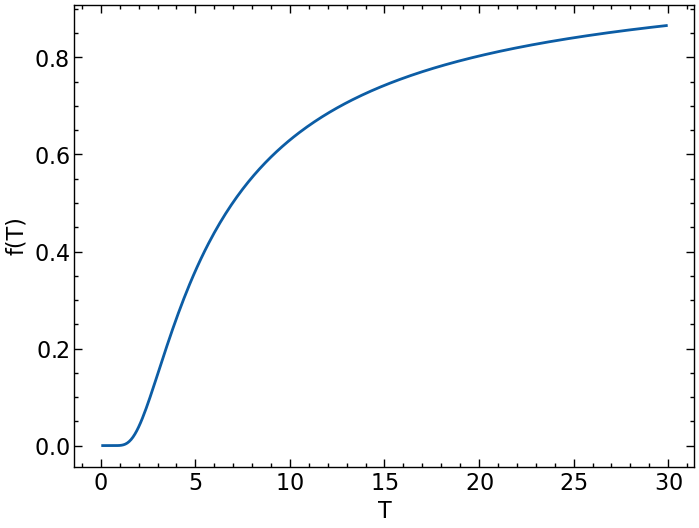
\includegraphics[width=0.5\paperwidth]{code/f_T.png}}
\end{figure}

\subsection{Restitution terms of the collision integrals}
The collision integrals for the restitutive terms read
\begin{equation}
    \begin{split}
        \avg{\pdv{t}(n_k\psi_k)}_r=\sum_{j}\alpha_{kj}\sigma_{kj}^2&\int
        \dd{\bg}\dd{\bV}e^{-A_{kj}V^2-B_{kj}g^2+R_{kj}\bV\vdot\bg}\Theta(g-\ltx{g}{agg})\\
        &\int\dd{\bn}\Theta\pqty{-\bg\vdot\bn}\abs{\bg\vdot\bn}\cdot
        \Delta\psi_k(\bV+\mu_j\bg)\Theta\pqty{\ltx{g}{frag}^2-(\bg\vdot\bn)^2},
    \end{split}
\end{equation}
where $\Delta\psi_k$ is the change of the physical value $\psi_k$ due to a single
restitutive collision. For the restitutive type of collisions, the number densities do not
change, since $\Delta(n_k)=0$. Hence we have only the temperature evolution term
\subsubsection{Temperature evolution inegrals for restitution}
Putting $\psi_k(\bv_k)=m_kv_k^2/2$, we have
\begin{equation}
    \avg{\pdv{t}\pqty{\frac{3}{2}n_k T_k}}_r=-\frac{1+\eps}{2}m_kn_k
    \sum_{j}\frac{\mu_jR_{kj}}{A_{kj}^2}F_{kj}\cdot n_j-
    \frac{1-\eps^2}{2}m_kn_k\sum_{j}\frac{\mu_j^2}{A_{kj}}F_{kj}\cdot n_j,
\end{equation}
where
\begin{equation}
    F_{kj}=2\sigma_{kj}^2C_{kj}^2\sqrt{\pi\pqty{u_i^2+u_j^2}}
    \pqty{A_{kj}\ltx{g}{frag}^4G^{(1)}_{kj}(\ltx{g}{frag},\infty)+
    A_{kj}G^{(5)}_{kj}(\ltx{g}{agg},\ltx{g}{frag})},
\end{equation}
where
\begin{equation}
    \begin{split}
        G^{(1)}_{kj}(\ltx{g}{frag},\infty)&=
        \int_{\ltx{g}{frag}}^{\infty}\dd{g}g\exp\pqty{-C_{kj}g^2}=
        \frac{1}{2C_{kj}^2}\exp\pqty{-C_{kj}\ltx{g}{frag}^2},\\
        G^{(5)}_{kj}(\ltx{g}{agg},\ltx{g}{frag})&=
        \int_{\ltx{g}{agg}}^{\ltx{g}{frag}}\dd{g}g^5\exp\pqty{-C_{kj}g^2}=\\
        &=\frac{1}{2C_{kj}^3}\bqty{\pqty{2+2C_{kj}\ltx{g}{agg}^2+C_{kj}^2\ltx{g}{agg}^4}
        \exp\pqty{-C_{kj}\ltx{g}{agg}^2}-
        \pqty{2+2C_{kj}\ltx{g}{frag}^2+C_{kj}^2\ltx{g}{frag}^4}
        \exp\pqty{-C_{kj}\ltx{g}{frag}^2}}.
    \end{split}
\end{equation}

\subsection{Fragmentation terms of the collision integrals}
The fragmentative terms of the collision integral reads
\begin{equation}
    \begin{split}
        \avg{\pdv{t}(n_k\psi_k)}_f=\sum_{i,j}\alpha_{ij}\sigma_{ij}^2&\int\dd{\bv_k}\int
        \dd{\bg}\dd{\bV}e^{-A_{ij}V^2-B_{ij}g^2+R_{ij}\bV\vdot\bg}\\
        &\int\dd{\bn}\Theta\pqty{-\bg\vdot\bn}\abs{\bg\vdot\bn}\cdot\psi_k(\bv_k)\cdot
        \Theta\pqty{(\bg\vdot\bn)^2-\ltx{g}{frag}^2}\times\\
        &\times\pqty{\delta_{k,1}\frac{i+j}{4\pi}\int\dd{\be}\delta\pqty{\bv_k-\bV-v'_c\be}
            -\delta_{k,i}\delta\pqty{\bv_k-\bv_i(\bg,\bV)}}.
    \end{split}
\end{equation}
Performing the actions of the delta functions, we have
\begin{equation}
    \begin{split}
        \avg{\pdv{t}(n_k\psi_k)}_f&=\frac{\delta_{k,1}}{4\pi}\sum_{i,j}(i+j)
        \alpha_{ij}\sigma_{ij}^2\int\dd{\bg}\dd{\bV}e^{-A_{ij}V^2-B_{ij}g^2+R_{ij}\bV\vdot\bg}\\
        &\int\dd{\bn}\Theta\pqty{-\bg\vdot\bn}\abs{\bg\vdot\bn}\cdot
        \Theta\pqty{(\bg\vdot\bn)^2-\ltx{g}{frag}^2}
        \int\dd{\be}\psi_k(\bV-v'_c\be)-\\
        &-\sum_{j}\alpha_{kj}\sigma_{kj}^2\int
        \dd{\bg}\dd{\bV}e^{-A_{kj}V^2-B_{kj}g^2+R_{kj}\bV\vdot\bg}\\
        &\int\dd{\bn}\Theta\pqty{-\bg\vdot\bn}\abs{\bg\vdot\bn}\cdot\psi_k(\bV+\mu_j\bg)\cdot
        \Theta\pqty{(\bg\vdot\bn)^2-\ltx{g}{frag}^2}.
    \end{split}
\end{equation}
\subsubsection{Number density evolution inegrals for fragmentation}
Again, putting $\psi_k=1$, we have
\begin{equation}
    \begin{split}
        \avg{\pdv{n_k}{t}}_f&=\delta_{k,1}\sum_{i,j}(i+j)
        \alpha_{ij}\sigma_{ij}^2\int\dd{\bg}\dd{\bV}
        e^{-A_{ij}V^2-B_{ij}g^2+R_{ij}\bV\vdot\bg}
        \int\dd{\bn}\Theta\pqty{-\bg\vdot\bn}\abs{\bg\vdot\bn}\cdot
        \Theta\pqty{(\bg\vdot\bn)^2-\ltx{g}{frag}^2}-\\
        &-\sum_{j}\alpha_{kj}\sigma_{kj}^2
        \int\dd{\bg}\dd{\bV}e^{-A_{kj}V^2-B_{kj}g^2+R_{kj}\bV\vdot\bg}
        \int\dd{\bn}\Theta\pqty{-\bg\vdot\bn}\abs{\bg\vdot\bn}\cdot
        \Theta\pqty{(\bg\vdot\bn)^2-\ltx{g}{frag}^2}.
    \end{split}
\end{equation}
Solving the angular integrals, we get
\begin{equation}
    \int\dd{\bn}\Theta\pqty{-\bg\vdot\bn}\abs{\bg\vdot\bn}\cdot
    \Theta\pqty{(\bg\vdot\bn)^2-\ltx{g}{frag}^2}=I_{\bn,f}^{1,0,0}(\bg)=
    \pi g\bqty{1-\pqty{\frac{\ltx{g}{frag}}{g}}^2}\Theta\pqty{g-\ltx{g}{frag}},
\end{equation}
hence
\begin{equation}
    \begin{split}
        \avg{\pdv{n_k}{t}}_f&=\delta_{k,1}\sum_{i,j}(i+j)4\pi^2
        \alpha_{ij}\sigma_{ij}^2\int_{\ltx{g}{frag}}^{\infty}
        \dd{g}g^3\bqty{1-\pqty{\frac{\ltx{g}{frag}}{g}}^2}
        \exp\pqty{-B_{ij}g^2}\int\dd{\bV}
        e^{-A_{ij}V^2+R_{ij}\bV\vdot\bg}-\\
        &-\sum_{j}4\pi^2\alpha_{kj}\sigma_{kj}^2
        \int_{\ltx{g}{frag}}^{\infty}\dd{g}g^3\bqty{1-\pqty{\frac{\ltx{g}{frag}}{g}}^2}
        \exp\pqty{-B_{ij}g^2}
        \int\dd{\bV}e^{-A_{kj}V^2+R_{kj}\bV\vdot\bg}.
    \end{split}
\end{equation}
The center of mass velocity integral is solved to give us
\begin{equation}
    \int\dd{\bV}\exp\pqty{-A_{kj}V^2+R_{kj}\bV\vdot\bg}=I_{\bV}^{0,0}(\bg)=
    \pqty{\frac{\pi}{A_{ij}}}^{3/2}\exp\pqty{\frac{R_{ij}^2}{4A_{ij}}\cdot g^2}.
\end{equation}
Now, we write the number density evolution integrals as
\begin{equation}
    \begin{split}
        \avg{\pdv{n_k}{t}}_f&=\delta_{k,1}\sum_{i,j}(i+j)4\pi^2\pqty{\frac{\pi}{A_{ij}}}^{3/2}
        \alpha_{ij}\sigma_{ij}^2\int_{\ltx{g}{frag}}^{\infty}
        \dd{g}g^3\bqty{1-\pqty{\frac{\ltx{g}{frag}}{g}}^2}
        \exp\pqty{-C_{ij}g^2}-\\
        &-\sum_{j}4\pi^2\pqty{\frac{\pi}{A_{ij}}}^{3/2}\alpha_{kj}\sigma_{kj}^2
        \int_{\ltx{g}{frag}}^{\infty}\dd{g}g^3\bqty{1-\pqty{\frac{\ltx{g}{frag}}{g}}^2}
        \exp\pqty{-C_{ij}g^2},
    \end{split}
\end{equation}
and opening the brackets we have
\begin{equation}
    \begin{split}
        \avg{\pdv{n_k}{t}}_f&=\delta_{k,1}\sum_{i,j}(i+j)4\pi^2\pqty{\frac{\pi}{A_{ij}}}^{3/2}
        \alpha_{ij}\sigma_{ij}^2\int_{\ltx{g}{frag}}^{\infty}
        \dd{g}g^3\exp\pqty{-C_{ij}g^2}-\\
        &-\delta_{k,1}\ltx{g}{frag}^2\sum_{i,j}(i+j)4\pi^2\pqty{\frac{\pi}{A_{ij}}}^{3/2}
        \alpha_{ij}\sigma_{ij}^2\int_{\ltx{g}{frag}}^{\infty}
        \dd{g}g\exp\pqty{-C_{ij}g^2}-\\
        &-\sum_{j}4\pi^2\pqty{\frac{\pi}{A_{ij}}}^{3/2}\alpha_{kj}\sigma_{kj}^2
        \int_{\ltx{g}{frag}}^{\infty}\dd{g}g^3\exp\pqty{-C_{ij}g^2}+\\
        &+\ltx{g}{frag}^2\sum_{j}4\pi^2\pqty{\frac{\pi}{A_{ij}}}^{3/2}\alpha_{kj}\sigma_{kj}^2
        \int_{\ltx{g}{frag}}^{\infty}\dd{g}g\exp\pqty{-C_{ij}g^2}.
    \end{split}
\end{equation}
Solving the incomplete Gaussian integrals
\begin{equation}
    \begin{split}
        G^{(1)}_{ij}(\ltx{g}{frag},\infty)&=\int_{\ltx{g}{frag}}^{\infty}
        \dd{g}g\exp\pqty{-C_{ij}g^2}=\frac{1}{2C_{ij}}\exp\pqty{-C_{ij}\ltx{g}{frag}^2},\\
        G^{(3)}_{ij}(\ltx{g}{frag},\infty)&=\int_{\ltx{g}{frag}}^{\infty}
        \dd{g}g^3\exp\pqty{-C_{ij}g^2}=
        \frac{1}{2C_{ij}^2}\pqty{1+C_{ij}\ltx{g}{frag}^2}\exp\pqty{-C_{ij}\ltx{g}{frag}^2},\\
    \end{split}
\end{equation}
we write
\begin{equation}
    \avg{\pdv{n_k}{t}}_f=\delta_{k,1}\sum_{i,j}(i+j)K^{fn}_{ij}n_in_j
    -\sum_{j}K^{fn}_{ij}n_in_j,
\end{equation}
where
\begin{equation}
    K^{fn}_{ij}=2\sigma_{kj}^2\sqrt{\pi\pqty{u_i^2+u_j^2}}
    \exp\pqty{-C_{ij}\ltx{g}{frag}^2}.
\end{equation}

\subsubsection{Temperature evolution inegrals for fragmentation}
By putting $\psi_k(\bv_k)=m_kv_k^2/2$, we have
\begin{equation}
    \begin{split}
        \avg{\pdv{t}\pqty{\frac{3}{2}n_kT_k}}_f&=\frac{\delta_{k,1}}{4\pi}\frac{m_k}{2}
        \sum_{i,j}(i+j)\alpha_{ij}\sigma_{ij}^2\int\dd{\bg}\dd{\bV}V^2
        e^{-A_{ij}V^2-B_{ij}g^2+R_{ij}\bV\vdot\bg}\\
        &\int\dd{\bn}\Theta\pqty{-\bg\vdot\bn}\abs{\bg\vdot\bn}\cdot
        \Theta\pqty{(\bg\vdot\bn)^2-\ltx{g}{frag}^2}+\\
        &+\frac{\delta_{k,1}}{4\pi}\frac{m_k}{2}
        \sum_{i,j}(i+j)\gamma_{ij}\alpha_{ij}\sigma_{ij}^2\int\dd{\bg}\dd{\bV}
        e^{-A_{ij}V^2-B_{ij}g^2+R_{ij}\bV\vdot\bg}\\
        &\int\dd{\bn}\Theta\pqty{-\bg\vdot\bn}\abs{\bg\vdot\bn}\pqty{\bg\vdot\bn}^2\cdot
        \Theta\pqty{(\bg\vdot\bn)^2-\ltx{g}{frag}^2}-\\
        &-\frac{m_k}{2}\sum_{j}\alpha_{kj}\sigma_{kj}^2\int
        \dd{\bg}\dd{\bV}e^{-A_{kj}V^2-B_{kj}g^2+R_{kj}\bV\vdot\bg}
        \pqty{V^2+\mu_j^2g^2+2\mu_j\pqty{\bV\vdot\bg}}\\
        &\int\dd{\bn}\Theta\pqty{-\bg\vdot\bn}\abs{\bg\vdot\bn}\cdot
        \Theta\pqty{(\bg\vdot\bn)^2-\ltx{g}{frag}^2},
    \end{split}
\end{equation}
where we have used $v'^2_c=\gamma_{ij}(\bg\vdot\bn)^2$. The angular integral parts are
\begin{equation}
    \int\dd{\bn}\Theta\pqty{-\bg\vdot\bn}\abs{\bg\vdot\bn}\cdot
    \Theta\pqty{(\bg\vdot\bn)^2-\ltx{g}{frag}^2}=I_{\bn,f}^{1,0,0}(\bg)=
    \pi g\bqty{1-\pqty{\frac{\ltx{g}{frag}}{g}}^2}\Theta\pqty{g-\ltx{g}{frag}},
\end{equation}
and
\begin{equation}
    \int\dd{\bn}\Theta\pqty{-\bg\vdot\bn}\abs{\bg\vdot\bn}\pqty{\bg\vdot\bn}^2\cdot
    \Theta\pqty{(\bg\vdot\bn)^2-\ltx{g}{frag}^2}=I_{\bn,f}^{1,2,0}=
    \frac{\pi g^3}{2}\bqty{1-\pqty{\frac{\ltx{g}{frag}}{g}}^4}\Theta\pqty{g-\ltx{g}{frag}}.
\end{equation}
Now we have
\begin{equation}
    \begin{split}
        \avg{\pdv{t}\pqty{\frac{3}{2}n_kT_k}}_f&=\delta_{k,1}\frac{m_k}{2}
        \sum_{i,j}(i+j)\pi\alpha_{ij}\sigma_{ij}^2\int_{\ltx{g}{frag}}^{\infty}
        \dd{g}g^3\bqty{1-\pqty{\frac{\ltx{g}{frag}}{g}}^2}e^{-B_{ij}g^2}
        \int\dd{\bV}V^2e^{-A_{ij}V^2+R_{ij}\bV\vdot\bg}-\\
        &-\delta_{k,1}\frac{m_k}{4}
        \sum_{i,j}(i+j)\gamma_{ij}\pi\alpha_{ij}\sigma_{ij}^2\int_{\ltx{g}{frag}}^{\infty}
        \dd{g}g^5\bqty{1-\pqty{\frac{\ltx{g}{frag}}{g}}^4}e^{-B_{ij}g^2}
        \int\dd{\bV}e^{-A_{ij}V^2+R_{ij}\bV\vdot\bg}-\\
        &-\frac{m_k}{2}\sum_{j}4\pi\alpha_{kj}\sigma_{kj}^2\int_{\ltx{g}{frag}}^{\infty}
        \dd{g}g^3\bqty{1-\pqty{\frac{\ltx{g}{frag}}{g}}^2}e^{-B_{kj}g^2}
        \int\dd{\bV}V^2e^{-A_{kj}V^2+R_{kj}\bV\vdot\bg}-\\
        &-\frac{m_k}{2}\sum_{j}\mu_j^2\cdot4\pi\alpha_{kj}\sigma_{kj}^2
        \int_{\ltx{g}{frag}}^{\infty}\dd{g}g^5
        \bqty{1-\pqty{\frac{\ltx{g}{frag}}{g}}^2}e^{-B_{kj}g^2}
        \int\dd{\bV}e^{-A_{kj}V^2+R_{kj}\bV\vdot\bg}-\\
        &-\frac{m_k}{2}\sum_{j}2\mu_j\cdot4\pi\alpha_{kj}\sigma_{kj}^2
        \int_{\ltx{g}{frag}}^{\infty}
        \dd{g}g^3\bqty{1-\pqty{\frac{\ltx{g}{frag}}{g}}^2}e^{-B_{kj}g^2}\int\dd{\bV}
        \pqty{\bV\vdot\bg}e^{-A_{kj}V^2+R_{kj}\bV\vdot\bg}.
    \end{split}
\end{equation}
The center of mass velocity integrals read
\begin{equation}
    \begin{split}
        I_{\bV}^{0,0}(\bu)&=\int\dd{\bV}\exp\pqty{-A_{ij}V^2+R_{ij}\bV\vdot\bg}=
        \pqty{\frac{\pi}{A_{ij}}}^{3/2}\exp\pqty{\frac{R_{ij}^2}{4A_{ij}}\cdot g^2},\\
        I_{\bV}^{1,0}(\bu)&=\int\dd{\bV}V^2\exp\pqty{-A_{ij}V^2+R_{ij}\bV\vdot\bg}=
        \pqty{\frac{\pi}{A_{ij}}}^{3/2}\frac{1}{A_{ij}}
        \exp\pqty{\frac{R_{ij}^2}{4A_{ij}}\cdot g^2}
        \pqty{\frac{R_{ij}^2}{4A_{ij}}\cdot g^2+\frac{3}{2}},\\
        I_{\bV}^{0,1}(\bu)&=\int\dd{\bV}(\bV\vdot\bg)
        \exp\pqty{-A_{ij}V^2+R_{ij}\bV\vdot\bg}=
        \frac{2}{R}\pqty{\frac{\pi}{A_{ij}}}^{3/2}\frac{R_{ij}^2g^2}{4A_{ij}}
        \exp\pqty{\frac{R_{ij}^2}{4A_{ij}}\cdot g^2}.
    \end{split}
\end{equation}
Using them, we write
\begin{equation}
    \begin{split}
        \avg{\pdv{t}\pqty{\frac{3}{2}n_kT_k}}_f&=\delta_{k,1}\frac{m_k}{2}
        \sum_{i,j}(i+j)\pqty{\frac{\pi}{A_{ij}}}^{5/2}\alpha_{ij}\sigma_{ij}^2
        \int_{\ltx{g}{frag}}^{\infty}
        \dd{g}g^3\bqty{1-\pqty{\frac{\ltx{g}{frag}}{g}}^2}
        \pqty{\frac{R_{ij}^2}{4A_{ij}}\cdot g^2+\frac{3}{2}}e^{-C_{ij}g^2}-\\
        &-\delta_{k,1}\frac{m_k}{4}
        \sum_{i,j}(i+j)\gamma_{ij}\pi\pqty{\frac{\pi}{A_{ij}}}^{3/2}
        \alpha_{ij}\sigma_{ij}^2\int_{\ltx{g}{frag}}^{\infty}
        \dd{g}g^5\bqty{1-\pqty{\frac{\ltx{g}{frag}}{g}}^4}e^{-C_{ij}g^2}-\\
        &-\frac{m_k}{2}\sum_{j}4\pqty{\frac{\pi}{A_{kj}}}^{5/2}\alpha_{kj}
        \sigma_{kj}^2\int_{\ltx{g}{frag}}^{\infty}
        \dd{g}g^3\bqty{1-\pqty{\frac{\ltx{g}{frag}}{g}}^2}
        \pqty{\frac{R_{kj}^2}{4A_{kj}}\cdot g^2+\frac{3}{2}}e^{-C_{kj}g^2}-\\
        &-\frac{m_k}{2}\sum_{j}\mu_j^2\cdot4\pi\pqty{\frac{\pi}{A_{kj}}}^{3/2}
        \alpha_{kj}\sigma_{kj}^2
        \int_{\ltx{g}{frag}}^{\infty}\dd{g}g^5
        \bqty{1-\pqty{\frac{\ltx{g}{frag}}{g}}^2}e^{-C_{kj}g^2}-\\
        &-\frac{m_k}{2}\sum_{j}2\mu_j\cdot4\pi\frac{2}{R_{kj}}
        \pqty{\frac{\pi}{A_{kj}}}^{3/2}\frac{R_{kj}^2}{4A_{kj}}\alpha_{kj}\sigma_{kj}^2
        \int_{\ltx{g}{frag}}^{\infty}
        \dd{g}g^5\bqty{1-\pqty{\frac{\ltx{g}{frag}}{g}}^2}e^{-C_{kj}g^2}.
    \end{split}
\end{equation}
Opening the brackets, we have
\begin{equation}
    \begin{split}
        \avg{\pdv{t}\pqty{\frac{3}{2}n_kT_k}}_f&=\delta_{k,1}\frac{m_k}{2}
        \sum_{i,j}(i+j)\pqty{\frac{\pi}{A_{ij}}}^{5/2}
        \bqty{\frac{R_{ij}^2}{4A_{ij}}-\frac{\gamma_{ij}A_{ij}}{2}}
        \alpha_{ij}\sigma_{ij}^2\int_{\ltx{g}{frag}}^{\infty}
        \dd{g}g^5e^{-C_{ij}g^2}-\\
        &-\delta_{k,1}\frac{m_k}{2}
        \sum_{i,j}(i+j)\pqty{\frac{\pi}{A_{ij}}}^{5/2}
        \bqty{\frac{R_{ij}^2}{4A_{ij}}\ltx{g}{frag}^2-\frac{3}{2}}
        \alpha_{ij}\sigma_{ij}^2
        \int_{\ltx{g}{frag}}^{\infty}
        \dd{g}g^3e^{-C_{ij}g^2}-\\
        &-\delta_{k,1}\frac{m_k}{2}
        \sum_{i,j}(i+j)\pqty{\frac{\pi}{A_{ij}}}^{5/2}
        \bqty{\frac{3}{2}\ltx{g}{frag}^2+\frac{\gamma_{ij}A_{ij}}{2}\ltx{g}{frag}^4}
        \alpha_{ij}\sigma_{ij}^2
        \int_{\ltx{g}{frag}}^{\infty}\dd{g}ge^{-C_{ij}g^2}-\\
        &-\frac{m_k}{2}\sum_{j}4\pqty{\frac{\pi}{A_{kj}}}^{5/2}
        \bqty{\frac{R_{kj}^2}{4A_{kj}}+\mu_j^2A_{kj}+\mu_jR_{kj}}
        \alpha_{kj}\sigma_{kj}^2\int_{\ltx{g}{frag}}^{\infty}
        \dd{g}g^5 e^{-C_{kj}g^2}+\\
        &+\frac{m_k}{2}\sum_{j}4\pqty{\frac{\pi}{A_{kj}}}^{5/2}
        \bqty{\pqty{\frac{R_{kj}^2}{4A_{kj}}+\mu_j^2A_{kj}+\mu_jR_{kj}}\cdot\ltx{g}{frag}^2
        -\frac{3}{2}}
        \alpha_{kj}\sigma_{kj}^2\int_{\ltx{g}{frag}}^{\infty}
        \dd{g}g^3e^{-C_{kj}g^2}+\\
        &+\frac{m_k}{2}\sum_{j}4\pqty{\frac{\pi}{A_{kj}}}^{5/2}
        \frac{3}{2}\ltx{g}{frag}^2\alpha_{kj}
        \sigma_{kj}^2\int_{\ltx{g}{frag}}^{\infty}
        \dd{g}ge^{-C_{kj}g^2}.
    \end{split}
\end{equation}
The incomplete Gaussian integrals are
\begin{equation}
    \begin{split}
        \int_{\ltx{g}{frag}}^{\infty}\dd{g}g e^{-C_{ij}g^2}&=
        \frac{1}{2C_{ij}}\exp\pqty{-C_{ij}\ltx{g}{frag}^2},\\
        \int_{\ltx{g}{frag}}^{\infty}\dd{g}g^3 e^{-C_{ij}g^2}&=
        \frac{1}{2C_{ij}^2}\pqty{1+C_{ij}\ltx{g}{frag}^2}\exp\pqty{-C_{ij}\ltx{g}{frag}^2},\\
        \int_{\ltx{g}{frag}}^{\infty}\dd{g}g^5 e^{-C_{ij}g^2}&=
        \frac{1}{2C_{ij}^3}\pqty{2+2C_{ij}\ltx{g}{frag}^2+C_{ij}^2\ltx{g}{frag}^4}
        \exp\pqty{-C_{ij}\ltx{g}{frag}^2},
    \end{split}
\end{equation}
and the fragmentative temperature evolution terms become
\begin{equation}
    \begin{split}
        \avg{\pdv{t}\pqty{\frac{3}{2}n_kT_k}}_f&=\delta_{k,1}\frac{m_k}{2}
        \sum_{i,j}(i+j)\pqty{\frac{\pi}{A_{ij}}}^{5/2}
        \bqty{\frac{R_{ij}^2}{4A_{ij}}-\frac{\gamma_{ij}A_{ij}}{2}}
        \alpha_{ij}\sigma_{ij}^2\frac{1}{2C_{ij}^3}\pqty{2+2C_{ij}\ltx{g}{frag}^2+C_{ij}^2
        \ltx{g}{frag}^4}\exp\pqty{-C_{ij}\ltx{g}{frag}^2}-\\
        &-\delta_{k,1}\frac{m_k}{2}
        \sum_{i,j}(i+j)\pqty{\frac{\pi}{A_{ij}}}^{5/2}
        \bqty{\frac{R_{ij}^2}{4A_{ij}}\ltx{g}{frag}^2-\frac{3}{2}}
        \alpha_{ij}\sigma_{ij}^2\frac{1}{2C_{ij}^2}\pqty{1+C_{ij}\ltx{g}{frag}^2}
        \exp\pqty{-C_{ij}\ltx{g}{frag}^2}-\\
        &-\delta_{k,1}\frac{m_k}{2}
        \sum_{i,j}(i+j)\pqty{\frac{\pi}{A_{ij}}}^{5/2}
        \bqty{\frac{3}{2}\ltx{g}{frag}^2+\frac{\gamma_{ij}A_{ij}}{2}\ltx{g}{frag}^4}
        \alpha_{ij}\sigma_{ij}^2\frac{1}{2C_{ij}}\exp\pqty{-C_{ij}\ltx{g}{frag}^2}-\\
        &-\frac{m_k}{2}\sum_{j}4\pqty{\frac{\pi}{A_{kj}}}^{5/2}
        \bqty{\frac{R_{kj}^2}{4A_{kj}}+\mu_j^2A_{kj}+\mu_jR_{kj}}
        \alpha_{kj}\sigma_{kj}^2
        \frac{1}{2C_{ij}^3}\pqty{2+2C_{ij}\ltx{g}{frag}^2+C_{ij}^2\ltx{g}{frag}^4}
        \exp\pqty{-C_{ij}\ltx{g}{frag}^2}+\\
        &+\frac{m_k}{2}\sum_{j}4\pqty{\frac{\pi}{A_{kj}}}^{5/2}
        \bqty{\pqty{\frac{R_{kj}^2}{4A_{kj}}+\mu_j^2A_{kj}+\mu_jR_{kj}}\cdot\ltx{g}{frag}^2
        -\frac{3}{2}}
        \alpha_{kj}\sigma_{kj}^2
        \frac{1}{2C_{ij}^2}\pqty{1+C_{ij}\ltx{g}{frag}^2}\exp\pqty{-C_{ij}\ltx{g}{frag}^2}+\\
        &+\frac{m_k}{2}\sum_{j}4\pqty{\frac{\pi}{A_{kj}}}^{5/2}
        \frac{3}{2}\ltx{g}{frag}^2\alpha_{kj}
        \sigma_{kj}^2\frac{1}{2C_{ij}}\exp\pqty{-C_{ij}\ltx{g}{frag}^2}.
    \end{split}
\end{equation}








\end{document}